% !TeX root = main.tex
%%%%%%%%%%%%%%%%%%%%%%%%% PREAMBLE %%%%%%%%%%%%%%%%%%%%%%%%%%%%%%%%
%%%%%%%%%%%%%%%%%%%%%%%% BASIC DOCUMENT SETUP %%%%%%%%%%%%%%%%%%%%%
\documentclass[a4paper]{report}
\usepackage[utf8]{inputenc}
\usepackage[english]{babel}

%%%%%%%%%%%%%%%%%%%%%%%%%% PACKAGES %%%%%%%%%%%%%%%%%%%%%%%%%%%%%%%
\usepackage{datetime}
\usepackage{datenumber}
\usepackage{parskip}
\usepackage{forest}
\usepackage{svg}        % makes it possible to use svg files
\usepackage{graphics}
\usepackage{multicol}
\usepackage{icomma}
\usepackage{microtype}  % microscopic typography refinement
\usepackage{lastpage}   % used to reference last page in footer
\usepackage{fancyhdr}   % Header
\usepackage{tcolorbox}
\usepackage{amssymb}
\usepackage[Bjornstrup]{fncychap}
\usepackage[titles]{tocloft}
\usepackage{amsmath}    % mathematics for matrices and more
\usepackage{amsfonts}
\usepackage{csquotes}
\usepackage{morewrites}

\usepackage{tikz}
\usetikzlibrary{calc}   % position og tikz labels
\usetikzlibrary{arrows.meta}
\usetikzlibrary{decorations.pathreplacing,calligraphy}

\usepackage{float}
\usepackage{pgfplots}
\pgfplotsset{compat=1.17}
\usepackage{xcolor}
\definecolor{blueplot}{RGB}{60, 64, 198}
\definecolor{yellowplot}{RGB}{255, 211, 42}
\definecolor{redplot}{RGB}{255, 63, 52}
\definecolor{greenplot}{RGB}{5, 196, 107}
\definecolor{greyplot}{RGB}{72, 84, 96}

\usepackage{siunitx}
\sisetup{%quotient-mode=fraction,
		output-decimal-marker = {,},
		per-mode = fraction,
		separate-uncertainty = true,
		multi-part-units=single,
		exponent-product = \cdot,
		range-phrase=--}
		
\usepackage{minted} % Syntax highlighting 
%\usemintedstyle{monokai}
\setminted[]{breaklines, 
    breakafter=d,
    frame=lines,
    framesep=2mm,
    baselinestretch=1.2,
    fontsize=\footnotesize,
    tabsize=4,
    linenos}


\makeatletter
\renewcommand\@makefnmark{\textsuperscript{[\@thefnmark]}}
\renewcommand\@makefntext[1]{\textsuperscript{[\@thefnmark]}\enspace #1}
\makeatother

\usepackage[hidelinks, linktoc=all]{hyperref} % links, references, \ref{...}
\hypersetup{
    colorlinks = true,
    linkcolor = blue,
    citecolor = blue,
    urlcolor = blue
}
\urlstyle{same}

\usepackage{todonotes}

\usepackage{subcaption}

\usepackage{forest}

\usepackage{lipsum}  

\usepackage{misc/quiver}

\usepackage{wrapfig}

\usepackage[export]{adjustbox}


\usepackage[pdf]{graphviz}

%%% Helper code for Overleaf's build system to
%%% automatically update output drawings when
%%% code in a \digraph{...} is modified
\usepackage{xpatch}
\makeatletter
\newcommand*{\addFileDependency}[1]{% argument=file name and extension
  \typeout{(#1)}
  \@addtofilelist{#1}
  \IfFileExists{#1}{}{\typeout{No file #1.}}
}
\makeatother
\xpretocmd{\digraph}{\addFileDependency{#2.dot}}{}{}

\usepackage[block=ragged, sorting=nyt, style=authoryear-ibid, backend=biber]{biblatex}
\setlength\bibitemsep{1.5\itemsep}
\addbibresource{misc/mybib.bib}

%%%%%%%%%%%%% ACTUAL VISIBLE CONTENT %%%%%%%%%%%%%%%%%%%%%%%%%%%%%%
\begin{document}
\begin{titlepage}
    \begin{centering}
    \vspace*{-20px}\large Department of Mathematics \& Computer Science\\
    University of Southern Denmark $|$ IMADA \\
    \today \\
    
    \vspace{\fill}
    
    \huge{\bf  Compiler for Panda} \\
    \Large{\bf BADM500: Bachelor Project}
    
    \vspace{\fill}
    
    \begin{minipage}{0.45\textwidth} 
    \begin{flushleft}
        \Large
        \textit{Author}\\
        KIAN BANKE LARSEN\\
        kilar20@student.sdu.dk
    \end{flushleft}
    \end{minipage}
    
    \vspace{\fill}
    
    \begin{minipage}{0.45\textwidth}
    \begin{flushleft}
        \Large
        \textit{Supervisor}\\
        KIM SKAK LARSEN\\
        Professor
    \end{flushleft}
    \end{minipage}
    
    \vspace{\fill}
    
    \includesvg[width=.4\textwidth]{misc/SDU.svg}
    
    \vspace*{0.1cm}
    
    \end{centering}
    
    \thispagestyle{empty}
\end{titlepage}

\pagenumbering{roman}

\begin{abstract}
\paragraph{English}
This paper examines the development of a simple compiler that makes use of several phases: scanning, parsing, symbol collection, desugaring, code generation, allocation and code emission. The scanner and parser are based on Python Lex-Yacc.

The main focus of the compiler implementation is register allocation, but the compiler has first been developed as a stack machine. It is therefore interesting to compare the performance of the two versions. It is concluded that the register machine achieves better performance than the stack machine, although it is unclear whether this is due to the liveness analysis and not just the use of faster instructions.

Choices and considerations have been made when necessary, which is why it is realized in retrospect that few things should have been done differently. The compiler implementation is based mainly on theory given in accompanying literature: \cite{ModernCompilerImplementation}, \cite{EnginneringACompiler} and SCIL known from DM565.

The compiler is publicly available here: \url{https://kianbankelarsen.github.io/Compiler/}.

\paragraph{Danish}
Rapporten undersøger udviklingen af en simpel compiler, der gør brug af flere faser: scanning, parsing, symbol collection, desugaring, code generation, allocation og code emission. Scanneren og parseren er baseret på Python Lex-Yacc. 

Hovedfokuset for compiler-implementationen er registerallokering, men først er compileren blevet udviklet som en stakmaskine. Det er herfor interessant at sammenligne performance af de to versioner. Det konkluderes at registermaskinen opnår bedre performance end stakmaskinen, dog er det uklart hvorvidt det skyldes liveness analysen og ikke bare brugen af hurtigere instruktioner.

Valg og overvejeler er gjort når det har været nødvendigt, hvorfor det er indset i retrospekt, at få ting bør have blevet gjort anderledes. Compiler-implementationen er baseret hovedsageligt på teori givet i følgende litteratur: \cite{ModernCompilerImplementation}, \cite{EnginneringACompiler} og SCIL kendt fra DM565. 

Compileren er offentlig tilgængelig her: \url{https://kianbankelarsen.github.io/Compiler/}.
\end{abstract}

{ \hypersetup{hidelinks} \tableofcontents \addtocontents{toc}{\vskip-40pt}}

\newpage
\pagenumbering{arabic}
\setcounter{page}{1}

\chapter{Introduction}
This paper examines how to make a simple compiler in Python, named Panda for no particular reason. The compiler is simple in the sense that some decisions have been made to ease the process, although the decisions are not necessarily optimal. The aim is to learn different compiler techniques and get a hands-on feel for the different compiler phases by actually implementing a working compiler, targeting X86 assembly. This is done using a Flex/Bison equivalent package such as \texttt{PLY} for scanning and parsing. 

The language to be compiled is a subset of the imperative language C. This has been chosen because of its simpler syntax and easy to read curly bracket enclosed static scopes. In this project, we are interested in making a language that supports integers and Booleans. The language must have control flow constructs in form of \texttt{if}-\texttt{else} statements and functions, and iterative constructs such as \texttt{for}- and \texttt{while}-loops. 

A modern compiler is, as is well known, divided into phases. These phases relate to lexical and syntactic analysis, resulting in an abstract syntax tree. Subsequent phases analyze and adorn the abstract syntax tree, building a symbol table and finally generating assembly code.

The main focus in regard to advanced techniques will be local register allocation, using techniques described in \cite{ModernCompilerImplementation}. Handling this efficiently requires data flow analysis via control-flow graph, construction of interference graph, graph coloring and translation back to instructions using a combination of the registers and the stack, when the available registers do not suffice.

Initially, a stack machine will be prepared, which will form the basis for developing a compiler that uses CPU registers. We will take advantage of the split phases property when replacing the stack code generation phase in favor of one that uses register allocation. This allows us to only worry about ensuring that subsequent phases are compatible with the changes made in the former phases.

When adding extra complexity such as register allocation, it is important to document the benefit of this choice. Performance of the stack machine and the register machine will therefore be constructively compared.

\chapter{Project Basics}
This section is reserved for articulating some choices made at the very beginning of the project that defines the framework for how to develop and use the compiler.

\section{Project Structure}
The \texttt{Compiler} module uses different Python packages -- things that belong together must be together. It has been desired to make a clear division between the different phases, and this has been achieved by creating the Python package \texttt{phase}. Likewise, \texttt{dataclass} is a package that contains internal data structures, in other words, classes used to hold data. \texttt{Printer} is a package that is used primarily for debugging, but sometimes it is just nice to consider data structures graphically. \texttt{Testing} is placed on the same level as \texttt{src} because it has nothing to do with the compiler's implementation, it is just a QA tool that makes it easier to verify correctness. \texttt{compiler.py} takes care of summarizing all functionality, but the module requires arguments from the command line, and those arguments (as well as testing) are handled in \texttt{main.py} (the project's main file). Moreover, a \texttt{README.md} has been written as a quick-start guide.

\begin{figure}[H]
    \centering
    \begin{subfigure}{0.3\textwidth}
    \centering
    \scalebox{0.65}{
\begin{forest}
  for tree={
    font=\ttfamily,
    grow'=0,
    child anchor=west,
    parent anchor=south,
    anchor=west,
    calign=first,
    edge path={
      \noexpand\path [draw, \forestoption{edge}]
      (!u.south west) +(7.5pt,0) |- node[fill,inner sep=1.25pt] {} (.child anchor)\forestoption{edge label};
    },
    before typesetting nodes={
      if n=1
        {insert before={[,phantom]}}
        {}
    },
    fit=band,
    before computing xy={l=15pt},
  }
[Compiler/
    [src/
        [dataclass/
            [AST.py]
            [iloc.py]
            [symbol.py]
        ]
        [printer/
            [ast\_printer.py]
            [generic\_printer.py]
            [symbol\_printer.py]
        ]
    ]
]
\end{forest}
}
    \end{subfigure}        
    \hfill
    \begin{subfigure}{0.3\textwidth}
    \centering
    \scalebox{0.7}{
\begin{forest}
  for tree={
    font=\ttfamily,
    grow'=0,
    child anchor=west,
    parent anchor=south,
    anchor=west,
    calign=first,
    edge path={
      \noexpand\path [draw, \forestoption{edge}]
      (!u.south west) +(7.5pt,0) |- node[fill,inner sep=1.25pt] {} (.child anchor)\forestoption{edge label};
    },
    before typesetting nodes={
      if n=1
        {insert before={[,phantom]}}
        {}
    },
    fit=band,
    before computing xy={l=15pt},
  }
[Compiler/
    [src/
        [printer/
            [ast\_printer.py]
            [generic\_printer.py]
            [symbol\_printer.py]
        ]
        [utils/]
        [compiler.py]
    ]
    [testing/
        [test-cases/]
        [test.py]
    ]
    [main.py]
    [README.md]
    [...]
]
\end{forest}
}
    \end{subfigure}
    \hfill
    \begin{subfigure}{0.3\textwidth}
    \centering
    \scalebox{0.65}{
\begin{forest}
  for tree={
    font=\ttfamily,
    grow'=0,
    child anchor=west,
    parent anchor=south,
    anchor=west,
    calign=first,
    edge path={
      \noexpand\path [draw, \forestoption{edge}]
      (!u.south west) +(7.5pt,0) |- node[fill,inner sep=1.25pt] {} (.child anchor)\forestoption{edge label};
    },
    before typesetting nodes={
      if n=1
        {insert before={[,phantom]}}
        {}
    },
    fit=band,
    before computing xy={l=15pt},
  }
[Compiler/
    [src/
        [utils/]
        [compiler.py]
    ]
    [testing/
        [test-cases/]
        [test.py]
    ]
    [main.py]
    [README.md]
    [...]
]
\end{forest}
}
    \end{subfigure}
    \caption{Project file tree.}
\end{figure}

\section{Python Lex-Yacc}
PLY is a native Python tool, relying on reflection, used to automatically generate scanners and LALR(1) parsers. The package is well documented at the following source: \cite{ply}. Usage of the package will be described when reviewing the compiler phases in isolation. It has been chosen to use PLY in order to reserve more time for the compiler itself, though studies show that most compilers use hand-coded scanners \parencite[69]{EnginneringACompiler}. However, tool-generated parsers are more common than hand-coded parsers \parencite[85]{EnginneringACompiler}.

\section{Design Principles \& Patterns}
When starting a new project, it is important to make some basic thoughts about the architecture. Sensible choices at the beginning can increase code readability and make maintainability easier. It is particularly important to consider design principles and design patterns, as this will have a big effect on, i.e., how data structures are traversed and code testability. In this context, design principles refer to SOLID, and design patterns refer to Gang of Four's 23 design patterns.

We will start by considering design principles. SOLID is a mnemonic acronym for a set of design principles concerning software development in object-oriented languages: \textbf{S}ingle Responsibility, \textbf{O}pen Closed, \textbf{L}iskov's Substitution, \textbf{I}nterface Segregation and \textbf{D}ependency Inversion. The principles are in many ways obvious when rehearsed, but not necessarily followed, as it requires active consideration. Single responsibility is particularly expressed in the project by the sharp division of phases and their interfaces between them. Open/closed is not particularly used in the project, as inheritance sparsely appears, though crucial in the \texttt{printer} package. It will never be necessary to edit the generic printer because functionality to print a specific data structure is first implemented upon extension. Liskov's substitution principle is accommodated in the AST data class, since any subtree is a valid tree and all nodes are AST nodes. Dependency inversion principle simply means that we must program against an interface and not an implementation. There is actually an incident where the project does not live up to this principle, and that is when using the hidden method \texttt{\_value2member\_map\_} on \texttt{Enum} in the parsing phase. Other examples apply, of course, as every class must accommodate every principle. This was just a quick review.

One of the big decisions regarding behavioral design patterns has been whether to use visitors, just like in the well known SCIL compiler from the DM565 course. It was decided not to use visitors because Python 3.10 comes with a new cool feature, namely the match statement, which makes it possible to exploit the benefits of structural pattern matching. Although it is nice to let the data structure decide its iteration, I still prefer having everything written explicitly when learning to write a compiler. Using match statements requires one to repeat the iteration logic for every new operation, but that somewhat also makes it easier to implement new logic, as one does not have to remember the visitor pattern. Another useful creational design pattern is the Singleton pattern used in \texttt{label\_generator.py}. This makes it possible to retrieve the label generator in any class, while preserving the state on \texttt{count}, without having to pass the object through all the phases manually.

\section{Compiler Usage}
The main file handles the instantiation and therefore also the running of the \texttt{PandaCompiler} class. Python \texttt{argparse} is used to take command line arguments because it adds a lot of user-friendliness to the compiler. \texttt{argparse} provides the opportunity to query the compiler usage in the terminal, thus showing what options are available. Doing so yields the result stated below:

\begin{minted}{text}
Compiler$ python3.10 main.py --help

usage: Compiler for Panda [-h] [-o OUTPUT] [-c] [-d] [-f FILE] [-t] [-r] [-s]

Compiles source code to assembly

options:
    -h, --help            show this help message and exit
    -o OUTPUT, --output OUTPUT
                        Name of assembly output file
    -c, --compile         Compile output with gcc
    -d, --debug           Debugging information, i.e., ILOC and Graphviz
    -f FILE, --file FILE  Path to input file; default is stdin.
    -t, --runTests        Run tests
    -r, --run             Run compilled program
    -s, --stack           Use stack only; default is registers
\end{minted}

This informs the user that one can specify an input file or provide input directly in the command line. Specifying the name of the output file is optional. Furthermore, one can control whether the file should be automatically compiled with \texttt{gcc} and directly run on the system. Many of the arguments act as flags to the compiler, such as \texttt{--debug} or \texttt{--runTests}, which are flags that specify whether a certain piece of code should be executed. Much of the \texttt{argparse} setup is omitted, in this example, but the essential part of the functionality is listed below. All pip requirements needed for running \texttt{main.py} can be installed using \texttt{pip install -r requirements.txt} -- file located in the root of the project.

\begin{minted}{py3}
args = argparser.parse_args()

if args.runTests:
    runner = unittest.TextTestRunner(verbosity=2)
    result = runner.run(testing.test.load_tests(args))
else:
    PandaCompiler(args).compile()
\end{minted}

If the \texttt{--runTests} flag is set, then it will take priority over the regular compiler functionality. However, it is still possible to specify \texttt{--debug}, as debugging information may be useful in case some tests fail. Debugging information is information such as graphical representation of data structures and pretty printed ILOC code -- sequential assembly IR. Testing will be explained in depth later.

\chapter{Phases}
One aspect that is important to consider is time. Keeping track of when various things happen is hard. 

\begin{displayquote}
    \textit{``Some decisions are made when the compiler is designed, at design time. Some algorithms run when the compiler is built, at build time. Many activities take place when the compiler itself runs, at compile time. Finally, the compiled code can execute multiple times, at runtime."}
\end{displayquote}
\hspace*\fill{\small--- \cite[8]{EnginneringACompiler}}

Clearly most time is spent on design time because it is at design time the compiler has been created in the development environment. This includes time spent on designing an interface and writing the code. Compile time is equally important, as it can be coded using more or less efficient algorithms. Perhaps the compiler depends on certain packages being available on the machine, just as various Python packages are used in this project. Some code has a very short lifetime in compile time before spending the rest of its life in runtime. It is therefore worth spending substantially more time during compile time in order to perform code analysis and subsequent optimization, such that the code running can be more efficient in some metric. The code could for example be optimized to run faster or save power. Fast programs are wanted when analyzing big data or fast response is needed. Focusing on power saving programs is key when targeting portable devices. 

A typical three-phase compiler is designed as shown in Figure \ref{fig:three-phase}.

\begin{figure}[H]
    \centering
    \begin{tikzpicture}
    \draw (-0.5, -0.5) rectangle ++(7.9, 2.25) node[anchor=north east, yshift=-1.7cm]{Compiler};
    \filldraw[fill=gray!20] (0,0) rectangle ++(1.9, 1.25) node[pos=.5]{Front End};
    \filldraw[fill=gray!20] (2.5,0) rectangle ++(1.9, 1.25) node[pos=.5]{Optimizer};
    \filldraw[fill=gray!20] (5,0) rectangle ++(1.9, 1.25) node[pos=.5]{Back End};
    \draw[->] (1.9, 0.625) -- ++(0.6, 0) node[midway, above]{IR};
    \draw[->] (4.4, 0.625) -- ++(0.6, 0) node[midway, above]{IR};
    \draw[->] (-2.5, 0.625) -- ++(2.5, 0) node[midway, align=center]{Source \\ program};
    \draw[->] (6.9, 0.625) -- ++(2.5, 0) node[midway, align=center]{Target \\ program};
\end{tikzpicture}
    \caption{Three-phase compiler.}
    \label{fig:three-phase}
\end{figure}

There is no restriction on what the individual stages can contain, as it depends entirely on architecture and program needs. The front end's responsibility is to understand the input program, such that it is possible to generate correct and meaningful code in the back end. The breakdown of Panda is presented in Figure \ref{fig:panda-structure}.

\begin{figure}[H]
    \centering
    \begin{tikzpicture}
    \draw (0, 0) rectangle ++(10.7, 6.25) node[anchor=north east, yshift=-5.75cm]{Compiler};
    \filldraw[fill=gray!20] (.5, .5) rectangle ++ (9.7, .5) node[pos=.5]{Shared Infrastructure};
    \filldraw[fill=gray!20] (.5, 1.25) rectangle ++(4.4, 4.5);
    \filldraw[fill=gray!20] (5.35, 1.25) rectangle ++(1.65, 4.5) node[pos=.5, yshift=.5cm]{$\emptyset$};
    \filldraw[fill=gray!20] (7.5, 1.25) rectangle ++(2.7, 4.5);
    \node[anchor=north west] at (.5, 5.75) {Front End};
    \node[anchor=north west] at (5.27, 5.75) {Optimizer};
    \node[anchor=north west] at (7.5, 5.75) {Back End};
    \filldraw[fill=white] (.75, 1.5) rectangle ++(.5, 3.5) node[pos=.5, rotate=90]{Scanner};
    \filldraw[fill=white] (1.6, 1.5) rectangle ++(.5, 3.5) node[pos=.5, rotate=90]{Parser};
    \filldraw[fill=white] (2.45, 1.5) rectangle ++(.5, 3.5) node[pos=.5, rotate=90]{Symbol Collection};
    \filldraw[fill=red!20] (3.3, 1.5) rectangle ++(.5, 3.5) node[pos=.5, rotate=90]{Type Checking};
    \filldraw[fill=white] (4.15, 1.5) rectangle ++(.5, 3.5) node[pos=.5, rotate=90]{Desugaring};
    \filldraw[fill=white] (7.75, 1.5) rectangle ++(.5, 3.5) node[pos=.5, rotate=90]{Code Generator};
    \filldraw[fill=blue!20] (8.6, 1.5) rectangle ++(.5, 3.5) node[pos=.5, rotate=90]{Allocator};
    \filldraw[fill=white] (9.45, 1.5) rectangle ++(.5, 3.5) node[pos=.5, rotate=90]{Emit};
    \draw[->] (0, 3.25) -- ++(0.75, 0);
    \draw[->] (1.25, 3.25) -- ++(0.35, 0);
    \draw[->] (2.1, 3.25) -- ++(0.35, 0);
    \draw[->] (2.95, 3.25) -- ++(0.35, 0);
    \draw[->] (3.8, 3.25) -- ++(0.35, 0);
    \draw[->] (4.65, 3.25) -- ++(3.1, 0);
    \draw[->] (8.25, 3.25) -- ++(0.35, 0);
    \draw[->] (9.1, 3.25) -- ++(0.35, 0);
    \draw[->] (9.95, 3.25) -- ++(0.75, 0);
    \draw[<->] (1, 1) -- ++(0, 0.5);
    \draw[<->] (1.85, 1) -- ++(0, 0.5);
    \draw[<->] (2.7, 1) -- ++(0, 0.5);
    \draw[<->] (3.55, 1) -- ++(0, 0.5);
    \draw[<->] (4.4, 1) -- ++(0, 0.5);
    \draw[<->] (8, 1) -- ++(0, 0.5);
    \draw[<->] (8.85, 1) -- ++(0, 0.5);
    \draw[<->] (9.7, 1) -- ++(0, 0.5);
\end{tikzpicture}
    \caption{Internal structure of Panda.}
    \label{fig:panda-structure}
\end{figure}

Type checking has been colored red because it has not been implemented yet, though it would be preferable to have functionality to refrain users from doing something nonsensical, for example, assigning a function to an integer variable.

\begin{minted}{c}
int a; int main(){} a = main;
\end{minted}

This error will cause the compiler to raise a value error during code generation, as the match statement for case \texttt{AST.StatementAssignment} is designed to do exactly that for any symbol with \texttt{NameCategory} parameter or variable -- function is neither. It is wanted that the compiler stops compiling on such error, but it should never crash because of an uncaught exception. The user must always be informed properly about what went wrong, without having to deal with an indifferent stack trace.

Optimizations like instruction selection, instruction scheduling and peephole etc. could have been interesting to implement, but this is unfortunately beyond the scope of this project, since time did not allow. The stage is therefore skipped.

Panda can either produce stack machine code or register machine code. The allocator phase is colored blue because it is clearly only used upon compiling source code to assembly code utilizing CPU registers. 

The individual phases presented in Figure \ref{fig:panda-structure} will be reviewed in detail in the subsequent sections of this chapter. As a consequence of having studied the SCIL compiler, it will be clear that several things are done similarly, or at least inspired by SCIL to some extent. 

\section{Scanning}
The scanner, or lexical analyzer, is the first phase of the compiler's front end. The scanner reads a stream of characters and produces a stream of words by aggregating the characters. For each word, it determines if the word is valid in the source language, and each valid word is assigned a syntactic category (corresponding to terminal symbols in the language's grammar) used by the parser. 

The scanner is the only phase in the compiler that touches every character of the source program. Because grouping characters is a simple task, scanners lend themselves to fast implementations. The Lex part of PLY is an automatic scanner generator tool. Lex requires a token list and specification of token values in order to produce a recognizer. The recognizer is based on a mathematical description of the language's lexical syntax in form of regular expressions and finite automatons. What method Lex uses to produce the scanner is unknown, but it can be achieved using Kleene's construction as presented in \cite[45]{EnginneringACompiler}.

The documentation for Lex can be found in \cite[section 4][]{ply}, and the guide is almost identical to the steps implemented in SCIL. The author of the tool tried to stay faithful to the way in which traditional Lex/Yacc tools work, so there was nothing surprising about how it should be done.

First, it is necessary to make a list of reserved words, as it would otherwise not be possible to separate them from regular identifiers, because reserved words are a subset of legal identifiers. The reserved words are something like \texttt{if}, \texttt{else}, \texttt{return} and so on. These are specified in Python using a dictionary with word as key and token as value.

\begin{minted}{py3}
reserved = {
    'print': 'PRINT',
    'return': 'RETURN',
    ...
}
\end{minted}

The immutable list of tokens is the union of tokens and reserved words. The list constitutes all valid words of the source program.

\begin{minted}{py3}
tokens = (
    'IDENT', 'INT', 'FLOAT',
    'PLUS', 'MINUS', 'TIMES', 'DIVIDE',
    ...
) + tuple(reserved.values())
\end{minted}

Rules for individual tokens are specified with a raw regex string as shown below:

\begin{minted}{py3}
t_PLUS = r'\+'
t_MINUS = r'-'
\end{minted}

The prefix \texttt{t\_} is used to indicate that it defines a token. The string must be compatible with Python's \texttt{re} module.

A token can also be specified as a function if some kind of action needs to be performed. This is particularly useful in connection with separating identifiers from reserved words. In that case, it will be possible to lookup a given identifier in reserved words. If the relevant key is not found, then it can be concluded that the token in question is just a regular identifier; otherwise, the found reserved token will be returned.

\begin{minted}{py3}
def t_IDENT(t):
    r'[a-zA-Z_][a-zA-Z_0-9]*'
    t.type = reserved.get(t.value, 'IDENT')
    return t
\end{minted}

This approach is recommended as it greatly reduces the number of regular expression rules.

\section{Parsing}
Parsing is the second phase of the compiler's front end. The parser's task is to determine whether a stream of tokenized words produced by the scanner constitutes a valid sentence in the programming language. The parser uses a context-free grammar to derive a syntactic structure for the program, fitting the tokenized words into the grammatical model. If the parser determines that the tokenized program is a valid program, it builds an intermediate representation (shortened IR). The resulting IR of this phase is a graphical IR, acyclic parse tree, because it encodes the program structure well.\footnote{We will consider the properties of a linear IR in section \ref{sec:code-gen}.} Choosing the correct IR has major consequences on what information can be encoded. It is necessary to have information encoded explicitly, as it is not possible to modify the implicit meaning of a structure.

The Yacc part of PLY uses a LALR(1) parser, which is a bottom-up parser, meaning that the parser will attempt to build a derivation bottom-up. Though we do not have to deal with the parser implementation, it is worth mentioning that top-down parsers are usually more intuitive, but bottom-up parsing is more practical and efficient for complex languages. 

The parser is used as a pull parser, meaning that the parser will request a new token whenever it is ready for more input. This is set up by letting the parser control both the input program and the lexer. 

\begin{minted}{py3}
src.phase.parser.parser.parse(
    user_program,
    lexer=src.phase.lexer.lexer
)
\end{minted}

The parsing result is provided by side effect, which is why the graphical IR can be retrieved by reading the variable called \texttt{interfacing\_program} located in \texttt{utils/\-interfacing\_parser.py}. 

The parser implementation has been done following the guidelines presented in \cite[section 6][]{ply}. Moreover, the grammar implemented is heavily inspired by how it was done in SCIL. 

The most prominently used idea is to store the entire program as a function that can be executed by the operating system by calling \texttt{main} -- the programs single access point. In this way, the idea of stack frames is already established, and the content of the program is thereby just the function body, which in turn can contain other function calls. The starting grammar rule is stated below:

\begin{minted}{py3}
def p_program(t):
    'program : body'
    interfacing_parser.the_program = AST.Function(
        "?main", None, t[1], t.lexer.lineno)
\end{minted}

Since the source program must be structured as specified by \texttt{Body}, it is interesting to see what fields are available.

\begin{minted}{py3}
@dataclass
class Body(AstNode):
    decls: DeclarationList
    stm_list: StatementList
    lineno: int    
\end{minted}

The \texttt{Body} class is annotated with \texttt{dataclass}. Python data classes are specially structured classes optimized for storage and representation, and it allows for concise class declaration since the constructor is generated automatically.

To make the language semantics easy to understand, it has been decided to constraint that declarations of variables must come before any usage. Declarations and statements are both optional (body can be empty), though useless without statements. Mixing declarations and statements can be confusing to handle, and it will be elaborated in section \ref{sec:symbol_collection} why it encourages trouble.

\begin{minted}{py3}
def p_body(t):
    'body : optional_declarations optional_statement_list'
    t[0] = AST.Body(t[1], t[2], t.lexer.lineno)
\end{minted}

Associativity of tokens can be encoded directly in the grammar, but can also be specified as precedence directives for the parser. It makes the grammar simpler when one can ignore this kind of trouble. The precedence directives stated below specify that the parser must reduce when encountering \texttt{TIMES}, \texttt{DIVIDE} etc. and shift when encountering \texttt{EQ}. The directives go from lowest to highest precedence. The \texttt{nonassoc} directive used on comparison based operators are very useful, because it refrains the user from specifying some like \texttt{3 < x < 7}. The semantic of this statement is powerful, although difficult to express directly in code, as it is syntactic sugar for two subsequent statements. The \texttt{nonassoc} directive will cause the parser to throw an error whenever it encounters such a case. 

\begin{minted}{py3}
precedence = (
    ('nonassoc', 'NEQ', 'LT', 'GT', 'LTE', 'GTE'),
    ('right', 'EQ'),
    ('left', 'PLUS', 'MINUS'),
    ('left', 'TIMES', 'DIVIDE')
)
\end{minted}

Parsing is a relatively large operation, but it was a representative sample.

To gain better insight into the resulting IR of the parsing phase, one can advantageously use the \texttt{printer} class to create a graphical representation of the AST data structure. We will consider the input program stated in Figure \ref{fig:ex_program}.

\begin{figure}[H]
\begin{minted}{c}
int j = 5; 
for(int i = 1; i < 5; i = i + 1){}   
\end{minted}
    \caption{Example program.}
    \label{fig:ex_program}
\end{figure}

The resulting abstract syntax tree is given in Figure \ref{fig:AST}.

\begin{figure}[H]
    \centering
    \digraph[scale=0.5]{ast}{
	0 [label="?main"]
	1 [label=body]
	2 [label=init_var_decl]
	3 [label=5]
	4 [label=int]
	5 [label=j]
	2 -> 4
	2 -> 5
	2 -> 3
	6 [label=decl_list]
	6 -> 2
	1 -> 6
	7 [label=stm_list]
	8 [label=init_var_decl]
	9 [label=1]
	10 [label=int]
	11 [label=i]
	8 -> 10
	8 -> 11
	8 -> 9
	12 [label=i]
	13 [label=5]
	14 [label="<"]
	14 -> 12
	14 -> 13
	15 [label=i]
	16 [label=1]
	17 [label="+"]
	17 -> 15
	17 -> 16
	18 [label="="]
	19 [label=i]
	18 -> 19
	18 -> 17
	20 [label=body]
	21 [label=for]
	21 -> 8
	21 -> 14
	21 -> 18
	21 -> 20
	7 -> 21
	1 -> 7
	0 -> 1
}

    \caption{Abstract Syntax Tree.} 
    \label{fig:AST}
\end{figure}

The input program stated in Figure \ref{fig:ex_program} is a good example because it is a small program with an associated small parse tree, although the parse tree is more verbose than it necessarily should be. Furthermore, there are two different uses of the \texttt{init\_var\_decl} vertex -- this vertex contains syntax such as \texttt{int i = 1;}. All usages of that vertex is syntactic sugar for a declaration and simultaneous assignment. The iterative \texttt{for} construction uses it as a parameter, so that it can just be transformed directly when visited. The story is a little more complicated for other usages of this vertex, since code for declarations is first generated after all statements belonging to a \texttt{body} vertex have been visited. It has therefore been necessary to add a desugaring phase to transform the AST, as we will see later in section \ref{sec:desugar}.

Panda is designed in such a way that every curly bracket enclosed environment creates a new scope. The default scope is global scope. Every scope consists of a single \texttt{body} vertex -- the grammar is \texttt{`new\_scope : LCURL body RCURL'}. Recall that a \texttt{body} vertex can contain optional declarations followed by optional statements. Just to mention Boolean values, the convention used is that the integer value $0$ is \texttt{false}; otherwise \texttt{true}.

The syntax is very C-like, but below are some examples of the different language constructions. Starting with a \texttt{for} loop:

\begin{minted}{c}
for(int i = 1; i < 5; i = i + 1){...}
\end{minted}

Then a \texttt{while} loops follow naturally:

\begin{minted}{c}
while(...){...}
\end{minted}

The \texttt{if}-\texttt{else} flow control statement:

\begin{minted}{c}
if(...){...} else{...}
\end{minted}

The classical \texttt{print} statement:

\begin{minted}{c}
print(3 + 5); 
\end{minted}

And finally function calls:\footnote{Remark: it is not valid to assign \texttt{void} function calls to any variable.}

\begin{minted}{c}
int a; int b = 1;
int fee(int arg){... return ...;}
void foo(){...}

a = fee(b);
foo();
\end{minted}

More examples can be found in the \texttt{/testing/test-cases/} folder.

\newpage

\section{Symbol Collection}\label{sec:symbol_collection}
Symbol collection is the third phase of the compiler's front end. The compiler discovers the names and properties of many entities during parsing. For each name used in the program, the compiler needs a variety of information before it can generate code to manipulate that entity. The Symbol Collection phase implements a recursive traversal of the AST in order to collect symbols into symbol tables.

Each scope has its own symbol table and each symbol within that scope is stored in that symbol table. The sole purpose of scopes is to encapsulate symbols so that logically separate parts of the program do not interfere. The introduction of scopes makes it possible to reuse symbol names, which is convenient, and a necessity when using recursion. The scoping mechanism implemented in Panda is static nested scoping. ``Static" because it can be determined where a symbol is accessible and visible by reasoning about the lexical structure of the source program -- this is often a cognitive comprehensive task when reading programs based on dynamic scoping. ``Nested" refers to the hierarchical separation of scopes. The primary purpose of a symbol table is to resolve names. When the compiler finds a symbol, it needs a mechanism that maps that symbol back to its declaration; otherwise we would not be able to locate the entity in memory.

The compiler for Panda only supports simple \SI{64}{bit} scalar variables and functions, and some additional information such as source register (\texttt{SR}) and \texttt{escaping} which will be elaborated in the Code Generation phase (section \ref{sec:register_machine}). The \texttt{Symbol} class is defined as stated in Figure \ref{fig:symbol}.

\begin{figure}[H]
\begin{minted}{py}
@dataclass
class Symbol:
    type: str
    kind: NameCategory
    info: int
    SR: int = None
    escaping: bool = False
\end{minted}
    \caption{Symbol to be stored in symbol table.}
    \label{fig:symbol}
\end{figure}

Each symbol encountered is stored in a symbol table associated with information about its \texttt{type}, \texttt{kind} (variable, parameter or function) and \texttt{info} (offset such that the variable can be located on the stack). The following has been inserted to provide insight into what happens when encountering a function declaration:

\begin{minted}{py3}
case AST.DeclarationFunction(type, func, lineno):
    symval = Symbol(type, NameCategory.FUNCTION, func)
    self._current_scope.insert(func.name, symval, lineno)
    self._current_scope = SymbolTable(self._current_scope)
    self._build_symbol_table(func)
case ...
\end{minted}

In this case, \texttt{\_current\_scope} is the active symbol table. It is thereby possible to instantiate a \texttt{Symbol} with information about the function and insert it into the table. Before recursively collecting symbols within that function, a new symbol table is instantiated for that scope.

The symbol table is declared as shown below:

\begin{minted}{py3}
@dataclass(init=False)
class SymbolTable:
    level: int
    parent: SymbolTable
    _tab: dict

    def __init__(self, parent: SymbolTable) -> SymbolTable:
        self._tab = {}
        self.level = parent.level + 1 if parent else 0
        self.parent = parent
\end{minted}

The symbol table itself keeps track of its lexical \texttt{level}, its parent, and the actual symbol table named \texttt{\_tab}. The \texttt{parent} field makes it possible to search upwards in the structure towards the global scope, if the symbol searched for is not at the current level.

Scopes create a tree structure, but where leafs point to the root and not the other way around. Considering the input program stated in Figure \ref{fig:ex_program} again, we see, in Figure \ref{fig:symbol_collection}, that \texttt{j} is declared in the global scope (root, level $0$) and \texttt{i} is declared at level $1$ immediately incident to global scope. 

\begin{figure}[H]
    \centering
    \digraph[scale=0.5]{symbol}{
	graph [rankdir=BT]
	0 [label=j]
	1 [label=i]
	1 -> 0
}

    \caption{Symbol collection.} 
    \label{fig:symbol_collection}
\end{figure}

Because the example just presented is relatively minimal, a more exciting input program is considered below:

\begin{minted}{c}
int a; 
if(3<4){int b;} else{int c; if(3){int c;} else{int d;}} 
while(4){int d;}
\end{minted}

It is here clearly shown how to quickly introduce some scopes by using \texttt{if}-\texttt{else} statements, since all curly bracket enclosed environments constitute a new scope. Furthermore, it is also noted that two versions of \texttt{d} are accessible in two respective scopes. 

\begin{figure}[H]
    \centering
    \digraph[scale=0.5]{symbol2}{
	graph [rankdir=BT]
	0 [label=a]
	1 [label=b]
	1 -> 0
	2 [label=c]
	2 -> 0
	3 [label=c]
	3 -> 2
	4 [label=d]
	4 -> 2
	5 [label=d]
	5 -> 0
}

    \caption{Another symbol collection example.} 
\end{figure}

The symbol collection figures are automatically generated using \texttt{printer/\-symbol\_printer.py}. The feature is only provided when executing the compiler with the debug option.

To return to the issue of mixing declarations and statements, it is quickly realized that this places greater demands on parser flexibility, since it will no longer be possible to make a discrete segregation of these groups. As such, it makes no difference to the symbol collection phase, as we already have to recurse through both declarations and statements. It will make code generation more complicated, because code for functions declared within the scope will be generated simultaneously with statements, if this is not handled with some special case logic. Besides, the mixing also makes it confusing to know which variable is accessed when, since some declaration can appear near the end of the scope -- the declaration is valid for the entire scope and not just after the line it appears. This is a hypothetical implementation, open for discussion, of course.

To give an example of what problems may arise with this implementation, please consider the code fragment below. The code fragment is a valid program using the hypothetical implementation, but it is difficult to determine which \texttt{a} is being referenced. This would have been harder to spot if the distance between the use and the declaration of \texttt{a} spanned multiple lines.

\begin{minted}{c}
void main(){print(a); int a = 8;}
a = 5;
main();
int a;
\end{minted}

\section{Desugaring}\label{sec:desugar}
Desugaring is the fourth, and last, phase of the compiler's front end. Desugaring is a phase that has been included because it was realized that the way nodes were visited during code generation was inexpedient, although necessary. The problem is only associated with the grammar:

\begin{center}
\texttt{variable\_init\_declaration : type IDENT ASSIGN expression SEMICOL}
\end{center}

Code for statements is produced before producing code for declarations. This is because we want to strangulate declared functions such that they do not appear within the function executed by the operating system. The functions would otherwise execute without being called by the user.

The way the problem has been solved is by traversing declarations and collecting all nodes of this type. The nodes are then transformed to \texttt{StatementAssignment} nodes and inserted, in the beginning and in the same order, as assignment statements too. The transformed nodes could have been advantageously removed from the tree, to minimize the IR, but since they do nothing, it has been decided to leave them as they are. The algorithmic approach is stated below:

\begin{minted}{py3}
case AST.Body(decls):
    self._desugar_AST(decls)
    decl_var_init_list = self._collect_decl_var_init(decls)
    assignments = self._trans_var_init_list_to_stm(decl_var_init_list)
    self._insert_stm(assignments, ast_node)
    self._desugar_AST(ast_node.stm_list)
\end{minted}

Reusing the input program from Figure \ref{fig:ex_program}, we can observe that the yellow nodes have been inserted, in Figure \ref{fig:desugar}, as a result of the desugaring phase.

\begin{figure}[H]
    \centering
    \digraph[scale=0.37]{desugar}{
	0 [label="?main"]
	1 [label=body]
	2 [label=init_var_decl]
	3 [label=5]
	4 [label=int]
	5 [label=j]
	2 -> 4
	2 -> 5
	2 -> 3
	6 [label=decl_list]
	6 -> 2
	1 -> 6
	7 [label=stm_list color="black" fillcolor="yellow" style=filled]
	8 [label=5 color="black" fillcolor="yellow" style=filled]
	9 [label="=" color="black" fillcolor="yellow" style=filled]
	10 [label=j color="black" fillcolor="yellow" style=filled]
	9 -> 10
	9 -> 8
	7 -> 9
	11 [label=stm_list]
	12 [label=init_var_decl]
	13 [label=1]
	14 [label=int]
	15 [label=i]
	12 -> 14
	12 -> 15
	12 -> 13
	16 [label=i]
	17 [label=5]
	18 [label="<"]
	18 -> 16
	18 -> 17
	19 [label=i]
	20 [label=1]
	21 [label="+"]
	21 -> 19
	21 -> 20
	22 [label="="]
	23 [label=i]
	22 -> 23
	22 -> 21
	24 [label=body]
	25 [label=for]
	25 -> 12
	25 -> 18
	25 -> 22
	25 -> 24
	11 -> 25
	7 -> 11
	1 -> 7
	0 -> 1
}

    \caption{Desugaring tree.} 
    \label{fig:desugar}
\end{figure}

\newpage

\section{Code Generation} \label{sec:code-gen}
Every process running on the computer is given a virtual address space. Figure \ref{fig:address_space} shows this. Here we note that there are four sections whose significance we should consider. Executable code lives in the \textit{code} section. Static contains statically defined entities -- not used for anything other than the \texttt{form} string specified in \texttt{emit.py}. The Panda programming language does not allow the programmer to define something statically. The \textit{heap} is for dynamically allocating memory, which unfortunately is also not possible in the Panda language. Our primary concern is therefore the \textit{stack}, since the stack contains all variables and information associated with procedure linkage.  

\begin{figure}[H]
    \centering
    \begin{tikzpicture}
    \node[anchor=south west] at (0, 2) {Low};
    \node[anchor=south east] at (8, 2) {$2^n$};
    \draw (0,0) rectangle ++(1, 2) node[rotate=90, pos=.5]{Code};
    \draw (1,0) rectangle ++(1, 2) node[rotate=90, pos=.5]{Static};
    \draw (2,0) rectangle ++(1, 2) node[rotate=90, pos=.5]{Heap};
    \draw (3,0) rectangle ++(4, 2) node[pos=.5]{Free Memory};
    \draw (7,0) rectangle ++(1, 2) node[rotate=90, pos=.5]{Stack};
    \draw[->, dashed] (3,1) --++ (0.75, 0);
    \draw[->, dashed] (7,1) --++ (-0.75, 0);
\end{tikzpicture}
    \caption{Virtual address-space layout.} 
    \label{fig:address_space}
\end{figure}

The stack is a memory area where it is possible to \texttt{push} and \texttt{pop} elements as needed. One can also choose to statically reserve an amount of memory for data storage. The stack only brings value when used properly and judiciously. It is therefore up to the compiler-writer how the stack is to be used. The actual stack architecture does not matter as long as one decides on a protocol and acts accordingly and consistently. However, the final stack architecture is very much controlled by procedure linkage, which limits the number of free choices, since certain things must be located on the stack, although the scheme is a free choice. The chosen stack architecture used in Panda is represented in Figure \ref{fig:stack}. The stack has been strategically divided into sections belonging to the different phases of the procedure linkage. In addition, addressing of significant pointers are shown. \texttt{RBP} (base pointer) and \texttt{RSP} (stack pointer) are used for immediate addressing of entities.

\begin{figure}[H]
    \centering
    \begin{tikzpicture}
    \node[anchor=south east, xshift=-0.1cm] at (0,0) {$2^n$};
    \node[anchor=north east, xshift=-0.1cm] at (0,5.25) {Low};
    \draw (0,0) rectangle ++(5, 0.75) node[pos=.5]{Parameter Area};
    \draw (0,0.75) rectangle ++(5, 0.75) node[pos=.5]{Caller-Save Area};
    \draw (0,1.5) rectangle ++(5, 0.75) node[pos=.5]{Caller's ARP};
    \draw (0,2.25) rectangle ++(5, 0.75) node[pos=.5]{Return Address};
    \draw (0,3) rectangle ++(5, 0.75) node[pos=.5]{Callee-Save Area};
    \draw (0,3.75) rectangle ++(5, 0.75) node[pos=.5]{Local Data Area};
    \draw (0,4.5) rectangle ++(5, 0.75) node[pos=.5]{Temporary Saves};
    \draw[->, dashed] (5.75, 5.25) --++ (-0.75, 0) node[right, xshift=.8cm]{\%RSP};
    \draw[->, dashed] (5.75, 3.75) --++ (-0.75, 0) node[right, xshift=.8cm]{\%RBP};
    \draw[->, dashed] (5.75, 0.75) --++ (-0.75, 0) node[right, xshift=.8cm]{$\text{\%RBP} + 128$};
    \draw [decorate, decoration = {calligraphic brace, raise=2pt, amplitude=5pt}] (0,0) --++  (0,2.25) node[midway, xshift=-1cm]{Precall};
    \draw [decorate, decoration = {calligraphic brace, raise=2pt, amplitude=5pt}] (0,2.25) --++  (0,0.75) node[midway, xshift=-1cm]{Call};
    \draw [decorate, decoration = {calligraphic brace, raise=2pt, amplitude=5pt}] (0,3) --++  (0,1.5) node[midway, xshift=-1cm]{Prolog};
\end{tikzpicture}
    \caption{Stack Frame.} 
    \label{fig:stack}
\end{figure}

The first thing the operating system does when executing an assembly program is to call its main function. As mentioned earlier, the entire program's entry point is wrapped as a function, which is why it will be necessary to focus on procedure linkage already now. There are clearly defined rules for which registers caller and callee must preserve. This agreement makes it possible to utilize all registers, since we are guaranteed that callee-registers are restored to the same state as when they were borrowed when the caller needs them. Figure \ref{fig:procedure} shows how procedure linkage is implemented in Panda. \texttt{Prolog} is responsible for saving callee-save registers and allocating space for local variables on the stack. \texttt{Precall} is responsible for putting arguments on the stack, if there are any, saving caller-save registers and making sure to set up static link pointer such that variables declared in other scopes can be accessed. \texttt{Postreturn} and \texttt{Epilog} are really just inverse processes of \texttt{Prolog} and \texttt{Precall} to restore registers and free allocated stack space.

\begin{figure}[H]
    \centering
    \begin{tikzpicture}
    \draw (0,0) rectangle ++(2, 0.75) node[pos=.5]{Epilog};
    \draw (0,0.75) rectangle ++(2, 1) node[pos=.5]{};
    \draw (0,1.75) rectangle ++(2, 0.75) node[pos=.5]{Postreturn};
    \draw (0,2.5) rectangle ++(2, 0.75) node[pos=.5]{Precall};
    \draw (0,3.25) rectangle ++(2, 1) node[pos=.5]{};
    \draw (0,4.25) rectangle ++(2, 0.75) node[pos=.5]{Prolog};

    \draw (4,1.25) rectangle ++(2, 0.75) node[pos=.5]{Epilog};
    \draw (4,2) rectangle ++(2, 1) node[pos=.5]{};
    \draw (4,3) rectangle ++(2, 0.75) node[pos=.5]{Prolog};

    \draw[<-] (1, 0.75) --++ (0, 1);
    \draw[<-] (1, 3.25) --++ (0, 1);
    \draw[->] (2, 2.5) -- (4, 3.75) node[above, midway, sloped]{Call};
    \draw[<-] (2, 2.5) -- (4, 1.25) node[below, midway, sloped]{Return};
    \draw[<-] (5, 2) --++ (0, 1);

    \node[anchor=south] at (1, 5) {Procedure $p$};
    \node[anchor=south] at (5, 3.75) {Procedure $q$};
\end{tikzpicture}
    \caption{Procedure linkage.} 
    \label{fig:procedure}
\end{figure}

The entire procedure linkage process is quite essential for the register machine, whereas the stack machine only needs a subset of the functionality. Because the stack machine uses the stack for everything, it is not necessary to save registers other than \texttt{RBP}; however, all register are saved anyway according to convention. The reason is that the final emit phase is reused for both the stack machine and the register machine.

We shcematically know how things should be done, we just have to express this in code. The graphical IR is no longer sufficient, which is why we need a linear IR. The linear IR, called ILOC in \cite[19]{EnginneringACompiler}, is very similar to the assembly code we want to output. The literature describes ILOC as an instruction set designed for the RISC architecture, since it uses the three-operand format,

\begin{align*}
\mathrm{add} \quad r_1, r_2 \rightarrow r_3 \quad \text{// example instruction}
\end{align*}

where $r_1$ and $r_2$ are used for calculation and the result is stored in $r_3$. However, CISC is based primarily on two-operand format (second operand is destructive using AT\&T). Therefore, a closely related IR is used instead. The actual implementation is given below. It should be no secret that this is the same implementation used in SCIL, however it has been rewritten to use Python \texttt{dataclasses}. An instruction thus consists of an opcode and some operands:

\begin{minted}{py3}
@dataclass(init=False)
class Instruction:
    opcode: Op
    args: list(Operand)

    def __init__(self, *args) -> Instruction:
        self.opcode = args[0]
        self.args = args[1:]
\end{minted}

An operand consists of a \texttt{target} and an addressing \texttt{mode}. Valid targets and modes are those specified in \texttt{Enum T} and \texttt{Enum M}, respectively. These classes are found in the file: \texttt{/src/enums/code\_generation\_enum.py}. This makes it possible to address, for example, registers directly or immediately.

\begin{minted}{py3}
@dataclass
class Operand:
    target: Target
    addressing: Mode
\end{minted}

Translating the AST to the linear ILOC IR thus yields a list of instructions as shown below. The smart thing about this IR is that needed information is explicitly represented -- it can be information such as which temporaries are used and their addressing. One can therefore easily perform analyses on the code by iterating through the list of instructions and using structural pattern matching to extract information. The register machine will pass this IR through the allocator phase in order to assign temporaries to physical registers before emitting code. The stack machine does not require further analysis, instead the list of instructions will simply be passed on to the emit phase which will emit assembly code.

\begin{minted}{py3}
[
    Instruction(opcode=<Op.LABEL: '7'>,
        args=(Operand(target=Target(spec=<T.MEM: 2>, val='main'),
                    addressing=Mode(mode=<M.DIR: 1>, offset=None)),)),
    Instruction(opcode=<Op.META: '8'>, args=(<Meta.PROLOG: 2>,)),
    ...
]
\end{minted}

It is time to provide some examples of code generation. Therefore, we consider how to access entities in external scopes. \texttt{\_follow\_static\_link}, shown below, solves this problem by repeatedly dereferencing the parent's base pointer (called ARP in Figure \ref{fig:stack}, an acronym for Activation Record Pointer). After the function has returned, \texttt{RSL} can be offset to access the desired entity. The only parameter the function requires is \texttt{symbol\_level}, and then it makes sure to follow the static link pointer the required number of times (based on the \texttt{\_current\_scope} field).

\begin{minted}{py3}
def _follow_static_link(self, symbol_level: int) -> int:
    level_difference = self._current_scope.level - symbol_level
    self._append_instruction(
        Instruction(Op.MOVE,
                    Operand(Target(T.RBP), Mode(M.DIR)),
                    Operand(Target(T.RSL), Mode(M.DIR)))
    )
    self._get_code_block_to_extend().extend(
        [Instruction(Op.MOVE,
                        Operand(Target(T.RSL), Mode(M.IRL, -7)),
                        Operand(Target(T.RSL), Mode(M.DIR)))
            for _ in range(level_difference)]
    )

    return level_difference
\end{minted}

\texttt{\_get\_code\_block\_to\_extend} is an auxiliary function used to solve a problem that arose in the code generation for the register machine, because it is necessary to preserve blocks of code such that liveness can be performed on one block of instructions at a time. Both \texttt{\_append\_instruction} and \texttt{\_get\_code\_block\_to\_extend} are annotated as abstract in \texttt{code\_generation\_base.py} and therefore defined individually in the classes that uses them. This is a consequence of the register machine and the stack machine not sharing the same structure of the generated code, precisely because code generated by the register machine is not completely linear, but instead a mixture of instructions and lists -- elaborated later.

A similar problem is removing stack frames. In the case of returns from deeply nested scopes, it is necessary to be able to remove several stack frames simultaneously; otherwise saved register values and the return address will not be in the expected place, which will cause segmentation fault. This is solved by iteratively generating code to tear down the individual stack frames by updating \texttt{RBP}. Now we just need to tear down the stack by moving \texttt{RBP} into \texttt{RSP}, and that is done as part of the epilogue. The code snippet below is an excerpt of \texttt{StatementReturn}.

\begin{figure}[H]
    \centering
\begin{minted}{py3}
    _, symbol_level = self._current_scope.lookup(func.name)
    level_difference = self._current_scope.level - symbol_level
    
    self._get_code_block_to_extend().extend(
        [Instruction(Op.MOVE,
                        Operand(Target(T.RBP), Mode(M.IRL, -7)),
                        Operand(Target(T.RBP), Mode(M.DIR)))
            for _ in range(level_difference-1)]
    )
    \end{minted}
    \caption{Tear down multiple stack frames if needed.}
    \label{fig:remove_stack_frames}
\end{figure}

The example below shows how to generate code for a function. The use of match statements contributes to a good overview because it is possible to observe the entire function at once. The steps come in linear order, exactly as we want the internal representation. A good approach when writing code for a construction is therefore to think about the flow for the construction in question, and then simply apply the individual steps in that particular order.

\begin{minted}{py3}
case AST.Function(body=body):
    ...
    self._ensure_labels(ast_node)
    self._append_instruction(
        Instruction(Op.LABEL,
                    Operand(Target(T.MEM, ast_node.start_label), Mode(M.DIR)))
    )
    self._prolog(body)
    self._generate_code(body.stm_list)
    self._append_instruction(
        Instruction(Op.LABEL,
                    Operand(Target(T.MEM, ast_node.end_label), Mode(M.DIR)))
    )
    self._epilog()
    self._append_instruction(Instruction(Op.META, Meta.RET))
    self._generate_code(body.decls)
    ...
\end{minted}

We do not care about the actual content of the function body because other match cases that handle those cases recursively are prepared. We just know that whatever instructions the body contains must be specified there. This approach is guaranteed to work by the invariant-based code generation scheme.

Invariants are conditions that we can rely on throughout the compiler. The benefit is that it is easier to implement new constructions when we know that we can rely on certain invariants. Invariants are established and maintained by following certain protocols such as the stack protocol. Below are stated some concrete Panda invariants:

\begin{itemize}
    \item The stack organization in the form of stack frames.
    \item For constructions with multiple operands, the operands are processed left-to-right. Actual arguments to functions are processed right-to-left.
    \item Function calls use the stack for all parameters.
    \item A function's return value is stored in \texttt{RAX}.
    \item \SI{64}{bits} are used for all types of values.
    \item Constructions consuming a number of operands pop them from the stack; the stack top is the last argument. This invariant is mostly related to the stack machine, but a similar approach has been taken in the register machine -- we just maintain a stack of temporary register.
    \item Constructions producing a result: The stack machine pushes the result onto the stack. The register machine moves the result into a new temporary. 
\end{itemize}

\subsection{Stack Machine}
It is not possible to review code generation for all constructions for the stack machine, and therefore the code snippet for \texttt{ExpressionBinop} below is representatively selected. We start by noting that the piece of code perfectly complies with the presented invariants, so the content should not be surprising.

A binary operation consists of a left and right child. The invariant promises to process operands left-to-right, and therefore the left child is called recursively before the right child is called recursively. The recursive calls return two values on the stack that the binary operation annotated by the vertex applies. Depending on the AST, it may be that the resulting value must be used to evaluate another vertex higher up the tree, and in that way the result propagates upwards.

Structural pattern matching is used to extract \texttt{binop}, \texttt{lhs} and \texttt{rhs} as their own variables. To limit the matching to arithmetic binary operations (not comparisons), an \texttt{if}-guard is used to check that binary operation is one of the enumerations in the list. As said, the two recursive calls return two values on the stack. These two values are popped into register 1 and register 2, respectively, after which the binary operation (opcode) is performed with register 1 and register 2 as operands. Because the operation is destructive, the result is saved in register 2, and this value is finally pushed onto the stack. The stack machine is quite worry-free in the sense that we do not have to keep track of both registers and the stack, as everything we need is just consistently on the stack. It is only required that we push and pop in the correct order.

\begin{minted}{py3}
case AST.ExpressionBinop(binop, lhs, rhs) if binop in [Op.ADD, Op.SUB, Op.DIV, Op.MUL]:
    self._generate_code(lhs)
    self._generate_code(rhs)

    self._append_instruction(
        Instruction(Op.POP,
                    Operand(Target(T.REG, 1), Mode(M.DIR)))
    )
    self._append_instruction(
        Instruction(Op.POP,
                    Operand(Target(T.REG, 2), Mode(M.DIR)))
    )
    self._append_instruction(
        Instruction(binop,
                    Operand(Target(T.REG, 1), Mode(M.DIR)),
                    Operand(Target(T.REG, 2), Mode(M.DIR)))
    )
    self._append_instruction(
        Instruction(Op.PUSH,
                    Operand(Target(T.REG, 2), Mode(M.DIR)))
    )
\end{minted}

The idea behind comparison binary operations is very similar, but there is a little extra logic to handle pushing $1$ when true and $0$ otherwise.

\subsection{Register Machine}\label{sec:register_machine}
Many of the techniques used in the stack machine can be transferred to the register machine. Instead of having a stack of values in the virtual address space used at runtime, we just maintain a stack of temporary registers at compile time. This makes it possible to keep track of which registers are included in various operations. As a starting point, we pretend that we have an infinite number of registers available, and it is therefore up to the allocation phase to map these to physical registers. This functionality is implemented by enriching the class with the two fields below. \texttt{\_reg\_count} is used to keep track of how many temporaries have been used and which unique temporary to use next. \texttt{\_reg\_stack} is just a list that we can pop and push values to. By only using push and pop we achieve a LIFO priority queue, also known as a stack.

\begin{minted}{py3}
_reg_count: int = 0
_reg_stack: list[int] = field(default_factory=list)
\end{minted}

To compare the stack machine with the register machine, we again give the example of \texttt{ExpressionBinop}. Two recursive calls are made to produce two temporaries on the stack. Next, we move the second temporary, \texttt{reg2}, into a new temporary because the binary operation is destructive. \texttt{push\_new\_reg\_count} takes care of incrementing \texttt{\_reg\_count} and pushing the temporary onto the temporary stack. When the binary operation has been performed, we know that the result is located in the new temporary and that it is at the top of the temporary stack, such that it can be used for subsequent operations.

\begin{figure}[H]
\begin{minted}{py3}
case AST.ExpressionBinop(binop, lhs, rhs) if binop in [Op.ADD, Op.SUB, Op.DIV, Op.MUL]:
    self._generate_code(lhs)
    self._generate_code(rhs)

    reg1 = self._reg_stack_pop()
    reg2 = self._reg_stack_pop()

    self._push_new_reg_count()

    self._append_instruction(
        Instruction(Op.MOVE,
                    Operand(Target(T.REG, reg2), Mode(M.DIR)),
                    Operand(Target(T.REG, self._reg_count), Mode(M.DIR)))
    )
    self._append_instruction(
        Instruction(binop,
                    Operand(Target(T.REG, reg1), Mode(M.DIR)),
                    Operand(Target(T.REG, self._reg_count), Mode(M.DIR)))
    )
\end{minted}
\caption{Code generation for binary operation.}
\label{fig:binop}
\end{figure}

Instead of letting values flow through the stack, they just flow through registers. However, these are managed using a stack at compile time, so in that way the methods for the register machine and the stack machine are very similar -- at least in a programming aspect.

The goal in this phase is, like in the register machine, to produce a linear IR. However, the allocation phase requires that the bracket structure be preserved, and therefore the result is a hybrid IR. The final IR therefore looks as indicated below. A hybrid IR means to combine both graphic and linear IRs to capture their strengths and avoid their weaknesses. A typical hybrid IR is a control-flow graph that uses a linear IR to represent blocks of code and a graph to represent the flow of control among those blocks. As a starting point, the resulting hybrid IR from this phase is not a control-flow graph, but it has all the prerequisites to become one. The final modifications will be done in the allocation phase.

\begin{minted}{text}
[
    instruction_1,
    instruction_2,
    [
        instruction_...,
        ..., 
        instruction_n
    ],
    instruction_n+1
]
\end{minted}

Some things have been changed to achieve the above. \texttt{\_append\_instruction} has been modified to always append the given instruction to the last list in \texttt{\_code}. Furthermore, symbols and scopes must be handled in order to be able to reuse temporaries for identifiers. To create a new symbol scope use \texttt{\_create\_new\_symbol\_scope} and \texttt{\_remove\_symbol\_scope} to remove it again. For each scope that is opened, in addition to handling symbols, a new empty list is appended to \texttt{\_code}:

\begin{minted}{py3}
self._code.append([])
\end{minted}

As a scope is closed, in addition to processing symbols, instruction lists will be merged. The list we are working with is thus at the end as long as it is active, and when the scope is closed it becomes part of the accumulated IR.

\begin{minted}{py3}
if len(self._code) >= 2:
    list_to_merge = self._code.pop()
    self._code[-1].append(list_to_merge)
\end{minted}

The described IR implementation is quite simple in itself, but it is complicated by the fact that its administration is included in another method. This is done because both methods are used in exactly the same places; however, it would have been more readable to keep them separate.

A symbol is adorned with \texttt{SR} (acronym for source register) and \texttt{escaping}, and it will now be explained why this is the case.

\texttt{SR} is stored on the symbol to keep track of which temporary any symbol belongs to. It becomes particularly relevant in \texttt{StatementAssignment}, because we want to keep all the values in registers, and it is therefore necessary to be able to lookup which temporary a value must be assigned to.

\texttt{Escaping} is used because we have to keep track of whether the values being assigned to belong to another scope. This is critical because if we choose to store the value in a register, but then return from the scope, then the value is lost. It therefore becomes necessary to keep track of which values must be written back to memory when a scope is removed. To keep the implementation simple, it is chosen, as a starting point, to always assign values that are not declared in the current scope back to memory immediately.

To put it in perspective, consider the example below. If a symbol is marked as \texttt{escaping} then the value is just written directly back to memory as in the stack machine. If the value is not marked \texttt{escaping}, then one of two cases applies. Either it is the first time the value is assigned, which is why it will have \texttt{SR=None}, and therefore a new temporary is created to hold the value. If the symbol already has been given a temporary, then we just assign directly to this.

\begin{minted}{py3}
case AST.StatementAssignment(lhs, rhs):
    ...
    reg = self._reg_stack_pop()

    if symbol.escaping:
        # Assign to memory
        ...
    else:
        # Assign to temporary
        match symbol:
            case dataclass_symbol.Symbol(SR=None):
                # Init temporary
                symbol.SR = self._new_reg()
                self._save_symbol(symbol)
                self._append_instruction(
                    Instruction(Op.MOVE,
                                Operand(Target(T.REG, reg),
                                        Mode(M.DIR)),
                                Operand(Target(T.REG, symbol.SR), Mode(M.DIR)))
                )
            case dataclass_symbol.Symbol(SR=SR):
                # Reuse temporary
                self._append_instruction(
                    Instruction(Op.MOVE,
                                Operand(Target(T.REG, reg),
                                        Mode(M.DIR)),
                                Operand(Target(T.REG, SR), Mode(M.DIR)))
                )
\end{minted}

\section{Allocation}
The liveness implementation is based on the literature \cite[218-223]{ModernCompilerImplementation} and the subsequent register allocation (graph coloring) is based on the literature \cite[235-238]{ModernCompilerImplementation}. 

There are many steps involved in register allocation. In order to make the process clear and provide an overview, each step has its own method, which also calls auxiliary methods. \texttt{perform\_register\_allocation} is the only method exposed by the \texttt{Allocator} class. The method is included below:

\begin{minted}{py3}
def perform_register_allocation(self, code: list[Instruction]) -> list[Instruction]:
    code = copy.deepcopy(code) # input is left untouched

    self._find_labels(code)
    self._control_flow(code)
    self._liveness_analysis(code)
    graph = self._build_graph(code)
    colors = self._color_graph(graph)
    code = self._flatmap(code)
    self._rename_registers(colors, code)

    return code
\end{minted}

We are only interested in doing liveness analysis for instructions that use temporaries, so structural pattern matching is used to filter these out. Structural Pattern matching makes it easy to determine whether a temporary is used in the first or second operand or both. We therefore do not have to do many conditional checks, because it is all given in the match case. 

The first step is to create a mapping between labels and the closest instruction that uses temporaries. This information is used when performing control-flow; otherwise, it is not known where the flow should continue when a jump instruction is encountered.

Creating control flow is about chaining instructions, so that any instruction points to the next instruction in the flow. Every instruction is given a successor and predecessor attribute, though it was later realized that the predecessor was not needed. The successor attribute is not strictly necessary, as we would be able to obtain the same information during the iteration in another way, but it makes the subsequent steps a bit nicer. Both successor and predecessor would have been strictly necessary if we had based the iteration on following these pointers, but due to the use of match statements, it was judged that it was easier to use a for each loop for the iteration. Due to the scope implementation, it has been necessary to limit the analysis to each introduced scope and not just functions, which is the ideal solution. It is not possible to ensure the flow when registers are saved and restored along the way. Consider Figure \ref{fig:flow_while} for an example of a flow graph. In Panda, the scope is wrapped around the entire \texttt{while} construction. The flow is therefore as shown in the figure, apart from the fact that \texttt{body} is of course made up of multiple instructions.

\begin{figure}[H]
    \centering
    % https://q.uiver.app/?q=WzAsNSxbMCwxLCJ3aGlsZSJdLFswLDIsImJvZHkiXSxbMCwzLCJqbXAiXSxbMCw0LCJcXHZkb3RzIl0sWzAsMCwiXFx2ZG90cyJdLFswLDFdLFsxLDJdLFsyLDAsIiIsMCx7ImN1cnZlIjo0fV0sWzIsM10sWzQsMF1d
\[\begin{tikzcd}
	\vdots \\
	while \\
	body \\
	jmp \\
	\vdots
	\arrow[from=2-1, to=3-1]
	\arrow[from=3-1, to=4-1]
	\arrow[curve={height=24pt}, from=4-1, to=2-1]
	\arrow[from=4-1, to=5-1]
	\arrow[from=1-1, to=2-1]
\end{tikzcd}\]
    \caption{Loop construction flow graph.}
    \label{fig:flow_while}
\end{figure}

The limited flow is particularly expressed in an \texttt{if} statement. Optimally (but still locally) the flow would look like shown in Figure \ref{fig:if}, where, depending on the \texttt{if} condition, the flow continues in \texttt{then} or \texttt{else} and finally in the common final node. In this way, liveness can be calculated for the entire graph. Unfortunately, the case is as shown in Figure \ref{fig:restriected}. The flow is the same (shown with dotted lines), but in relation to the analysis, we just take the direct route through the statement. \texttt{then} and \texttt{else} will be their own scopes, and therefore they will have their own local flow isolated from their surroundings. This is by no means desired, but it is a consequence of a choice made early in the process, because it standardized scopes and made it possible to declare variables in all scopes.

\begin{figure}[H]
    \centering
    \begin{subfigure}{0.49\textwidth}
        \centering
        % https://q.uiver.app/?q=WzAsNixbMSwxLCJpZiJdLFsyLDIsImVsc2UiXSxbMCwyLCJ0aGVuIl0sWzEsMywiXFxidWxsZXQiXSxbMSwwLCJcXHZkb3RzICJdLFsxLDQsIlxcdmRvdHMiXSxbNCwwXSxbMCwyXSxbMiwzXSxbMCwxXSxbMSwzXSxbMyw1XV0=
\[\begin{tikzcd}
	& {\vdots } \\
	& if \\
	then && else \\
	& \bullet \\
	& \vdots
	\arrow[from=1-2, to=2-2]
	\arrow[from=2-2, to=3-1]
	\arrow[from=3-1, to=4-2]
	\arrow[from=2-2, to=3-3]
	\arrow[from=3-3, to=4-2]
	\arrow[from=4-2, to=5-2]
\end{tikzcd}\]
        \caption{\textit{Optimal} flow.}
        \label{fig:if}
    \end{subfigure}
    \begin{subfigure}{0.49\textwidth}
        \centering
        % https://q.uiver.app/?q=WzAsNixbMSwxLCJpZiJdLFsyLDIsImVsc2UiXSxbMCwyLCJ0aGVuIl0sWzEsMywiXFxidWxsZXQiXSxbMSwwLCJcXHZkb3RzICJdLFsxLDQsIlxcdmRvdHMiXSxbNCwwXSxbMyw1XSxbMCwzXSxbMCwyLCIiLDAseyJzdHlsZSI6eyJib2R5Ijp7Im5hbWUiOiJkb3R0ZWQifX19XSxbMiwzLCIiLDAseyJzdHlsZSI6eyJib2R5Ijp7Im5hbWUiOiJkb3R0ZWQifX19XSxbMCwxLCIiLDAseyJzdHlsZSI6eyJib2R5Ijp7Im5hbWUiOiJkb3R0ZWQifX19XSxbMSwzLCIiLDAseyJzdHlsZSI6eyJib2R5Ijp7Im5hbWUiOiJkb3R0ZWQifX19XV0=
\[\begin{tikzcd}
	& {\vdots } \\
	& if \\
	then && else \\
	& \bullet \\
	& \vdots
	\arrow[from=1-2, to=2-2]
	\arrow[from=4-2, to=5-2]
	\arrow[from=2-2, to=4-2]
	\arrow[dotted, from=2-2, to=3-1]
	\arrow[dotted, from=3-1, to=4-2]
	\arrow[dotted, from=2-2, to=3-3]
	\arrow[dotted, from=3-3, to=4-2]
\end{tikzcd}\]
        \caption{Restricted flow.}
        \label{fig:restriected}
    \end{subfigure}
    \caption{\texttt{if} construction flow graph.}
\end{figure}

Liveness analysis is about determining which temporaries are live at the same time. It is crucial in register allocation, because if two variables are not live at the same time, then they can share a register; otherwise, they must necessarily claim their own register. We say a temporary is live if it holds a value that may be needed in the future, so this analysis is called \textit{liveness} analysis. We obtain this information using the fixed point algorithm given in \cite[221]{ModernCompilerImplementation}. The implementation of this algorithm is given below:

\begin{minted}{py3}
def _liveness_analysis(self, code: list) -> None:
    change = True

    while (change):
        change = False

        for ins in reversed(code):
            if self._do_set_calc(ins):
                change = True
\end{minted}

Note that the instructions are parsed in reverse order. This is because the uses of a temporary come after its declaration. It's just a way to achieve fixed point faster. The algorithm works by preparing an \texttt{in} and \texttt{out} set for each instruction in the flow. The \texttt{in} set contains all the temporaries that are live for the instruction in question. \texttt{out} contains all the temporaries that must be taken care of for the next instruction. The algorithm keeps repeating the analysis of the flow until there are no changes to the \texttt{in} set. Worst-case run time of this algorithm is $O(N^4)$, \cite[224]{ModernCompilerImplementation}. 

To give intuition for the calculation of \texttt{in} and \texttt{out} sets, consider Figure \ref{fig:in-out-flow}. In the figure, an arbitrary vertex from the flow is considered, where it is indicated how the \texttt{in} and \texttt{out} sets follow the flow. Two \texttt{out} edges are specified because it may be that there is a conditional jump.

\begin{figure}[H]
    \centering
    \begin{tikzpicture}
    \draw (0,0) circle (0.5) node[align=center, xshift=.9cm]{use,\\def};
    \draw[<-] (0, -2) -- ++ (0, 1.5) node[midway, right]{out};
    \draw[<-] (0, 0.5) -- ++ (0, 1.5) node[midway, right]{in};
    \draw[->] (0,-0.5) -- (0,-0.5) arc[start angle=0, end angle=-90,radius=1.5cm] node[above]{out};
\end{tikzpicture}
    \caption{Abstract flow graph.}
    \label{fig:in-out-flow}
\end{figure}

\texttt{in} and \texttt{out} sets must be calculated for every vertex in the flow. This is done by using the dataflow equations in Figure \ref{fig:dataflow-eq} -- utilized in the \texttt{\_do\_set\_calc} method. Also, note how the definition of a temporary kills its liveliness. This is expected behavior because if there are no uses of a definition, then we can simply remove those instructions. Executing useless instructions is useless. 

\begin{figure}[H]
    \begin{align*}
        \mathrm{in}[n] &= \mathrm{use}[n] \cup (\mathrm{out}[n] - \mathrm{def}[n])\\
        \mathrm{out}[n] &= \bigcup\limits_{s \in \mathrm{succ}[n]} \mathrm{in}[s]
    \end{align*}
    \caption{Dataflow equations for liveness analysis.}
    \label{fig:dataflow-eq}
\end{figure}

To take a concrete example, consider the register allocation process for the input program below.

\begin{minted}{c}
int a = 5; int b = 7; print(a + b);
\end{minted}

We skip control-flow because the phase does not provide any information to display. The liveness analysis produces the \texttt{in} sets below. We only consider instructions that use temporaries, and these instructions are extracted (left) and associated with their \texttt{in} set (right).

\begin{minted}{text}
movq $1, r1:    {}
movq r1, r2:    {1}   
movq $7, reg3:  {2}   
movq r3, r4:    {2, 3}
movq r2, r5:    {2, 4}
addq r4, r5:    {4, 5}
push r5:        {5}
\end{minted}

Based on all these \texttt{in} sets, an interference graph is created. The graph is made by adding an edge between any pair of temporaries that share an \texttt{in} set. The implementation in Panda makes use of a dictionary to create a mapping (temporary: adjacency set) to represent a graph. The literature suggests making an interference matrix, but it immediately seemed easier to implement the graph with adjacency sets, as the graph has to be strangulated and assembled again during coloring.

\begin{minted}{py3}
[{1: set(), 2: {3, 4}, 3: {2}, 4: {2, 5}, 5: {4}}]
\end{minted}

The graph is drawn in Figure \ref{fig:interference-graph}.

\begin{figure}[H]
    \centering
    % https://q.uiver.app/?q=WzAsNSxbMCwwLCJUXzEiXSxbMiwwLCJUXzIiXSxbNCwwLCJUXzUiXSxbMiwyLCJUXzQiXSxbMCwyLCJUXzMiXSxbMywwLCIiLDAseyJzdHlsZSI6eyJoZWFkIjp7Im5hbWUiOiJub25lIn19fV0sWzMsMSwiIiwyLHsic3R5bGUiOnsiaGVhZCI6eyJuYW1lIjoibm9uZSJ9fX1dLFszLDIsIiIsMix7InN0eWxlIjp7ImhlYWQiOnsibmFtZSI6Im5vbmUifX19XSxbNCwzLCIiLDIseyJzdHlsZSI6eyJoZWFkIjp7Im5hbWUiOiJub25lIn19fV0sWzAsMSwiIiwwLHsic3R5bGUiOnsiaGVhZCI6eyJuYW1lIjoibm9uZSJ9fX1dLFsxLDIsIiIsMCx7InN0eWxlIjp7ImhlYWQiOnsibmFtZSI6Im5vbmUifX19XV0=
\[\begin{tikzcd}
	{T_1} && {T_2} && {T_5} \\
	\\
	{T_3} && {T_4}
	\arrow[no head, from=3-3, to=1-1]
	\arrow[no head, from=3-3, to=1-3]
	\arrow[no head, from=3-3, to=1-5]
	\arrow[no head, from=3-1, to=3-3]
	\arrow[no head, from=1-1, to=1-3]
	\arrow[no head, from=1-3, to=1-5]
\end{tikzcd}\]
    \caption{Interference graph.}
    \label{fig:interference-graph}
\end{figure}

Graph coloring is done using a simple heuristic, called Coloring by Simplification, in the following way:

\begin{enumerate}
    \item Suppose the graph $G$ has a vertex $m$ with fewer than $K$ neighbors, where $K$ is the number of registers on the machine.
    \item Let $G'$ be the graph obtained by removing $m$ from $G$.
    \item When a new vertex $m$ is added to the colored graph $G'$, it is assigned the lowest numbered color that is not assigned to any of its neighbors. If the neighbors of $m$ have at most $K-1$ colors among them, then a free color can always be found for $m$.
\end{enumerate}

This leads to a stack-based algorithm for coloring: we repeatedly remove (and push on a stack) nodes of degree less than $K$. Each such simplification leads to more opportunity for simplification. If it is not the case that there is a node with degree less than $K$, then a random vertex is chosen in the graph. There are many heuristics that can be used, and one of them is the highest degree first heuristic because they are more likely to require a new color. The implementation in Panda just randomly picks a vertex with degree lower than $K$, and if there is no such vertex, then a random vertex with degree $K$ or higher. The coloring implementation is provided below. $K = 10$ in Panda.

\begin{minted}{py3}
def _color_graph(self, graphs: list[defaultdict]) -> dict[int, int]:
    colors = defaultdict(lambda: None)

    for graph in graphs:
        stack = self._take_graph_apart(graph)
        self._assign_colors(stack, colors)

    return colors
\end{minted}

Running the algorithm on the input yields the color mapping (temporary: color) given below. The highest degree first heuristic would have colored the graph using only two colors, whereas we require three registers.

\begin{minted}{py3}
{5: 1, 4: 2, 3: 1, 2: 3, 1: 1}
\end{minted}

The graph in Figure \ref{fig:interference-graph} has been colored with the calculated colors in Figure \ref{fig:colored-interference-graph}.

\begin{figure}[H]
    \centering
    % https://q.uiver.app/#q=WzAsNSxbMiwwLCJcXGNvbG9ye2dyZWVufXtUXzJ9Il0sWzAsMCwiXFxjb2xvcntyZWR9e1RfMX0iXSxbMiwyLCJcXGNvbG9ye3JlZH17VF8zfSJdLFs0LDIsIlxcY29sb3J7Ymx1ZX17VF80fSJdLFs0LDAsIlxcY29sb3J7cmVkfXtUXzV9Il0sWzQsMywiIiwwLHsic3R5bGUiOnsiaGVhZCI6eyJuYW1lIjoibm9uZSJ9fX1dLFszLDAsIiIsMCx7InN0eWxlIjp7ImhlYWQiOnsibmFtZSI6Im5vbmUifX19XSxbMiwwLCIiLDIseyJzdHlsZSI6eyJoZWFkIjp7Im5hbWUiOiJub25lIn19fV1d
\[\begin{tikzcd}
	{\color{redplot}{T_1}} && {T_2} && {\color{redplot}{T_5}} \\
	\\
	&& {\color{redplot}{T_3}} && {\color{blueplot}{T_4}}
	\arrow[no head, from=1-5, to=3-5]
	\arrow[no head, from=3-5, to=1-3]
	\arrow[no head, from=3-3, to=1-3]
\end{tikzcd}\]
    \caption{Colored interference graph.}
    \label{fig:colored-interference-graph}
\end{figure}

\section{Emission}
The Emit phase is the last phase in the compiler's back end. It is in this phase that the internal representation introduced in the code generation is made into actual assembly instructions, which can then be compiled into machine code using \texttt{gcc}. Luckily it has been possible to develop an interface such that this class could be used for both the stack machine and register machine.

The mapping from the internal representation is almost 1:1. There are small deviations such as the use of \texttt{\%RSL}, which is a virtual register used to calculate links, but \texttt{RSL} does not exist natively on the x86 architecture. In addition, it is necessary to handle a handful of \texttt{Meta} instructions, because it made sense to assemble these into composite instructions, and then let the Emit phase handle the actual code for this, since it is the same every time -- these instructions could as well have been represented in the linear IR. The \texttt{Meta} instructions are:

\begin{minted}{py3}
self._enum_to_method_map = {
    Meta.CALL_PRINTF: self._call_printf,
    Meta.PROLOG: self._prolog,
    Meta.EPILOG: self._epilog,
    Meta.PRECALL: self._precall,
    Meta.POSTRETURN: self._postreturn,
    Meta.RET: self._ret
}
\end{minted}

The \texttt{Meta} instructions are thus simply mapped using a dictionary in Python, mapping the \texttt{Enum} to a function implemented within the Emit class.

The majority of these functions are used during procedure linkage, which is why it makes sense to declare exactly which registers are callee-save and caller-save registers:

\begin{minted}{py3}
self._callee_save_reg = ["rbx", "r12", "r13", "r14", "r15", "rbp"]
self._calleer_save_reg = ["rcx", "rdx", "rsi", "rdi", "r8", "r9", "r10", "r11"]
\end{minted}

It might also have been advantageous to specify these fields in another class, so that variable offsets did not have to be hard-coded in the code generation, but could instead have been implemented as a function on the two lists. Adding extra callee-save registers and caller-save registers would then not require further intervention than adding them to the correct list.

\texttt{Meta.CALL\_PRINTF} uses labels to ensure correct memory alignment, and we therefore want to reuse the \texttt{Labels} object instantiated during code generation. This is achieved using the property that the class is declared singleton, and Python will therefore just return the same instance as used in code generation, without manually having to pass that instance to \texttt{Emit}:

\begin{minted}{py3}
self._labels = Labels()
\end{minted}

It is important that the counter within \texttt{Labels} is not reset, since this could, in the worst case, cause clashing labels, meaning that the program would be incorrect and in turn prevent \texttt{gcc} from being able to compile it, since labels are no longer ensured to be unique.

The code snippet given below is responsible for ``dispatching'' any ILOC instruction to an assembly instruction. Because the ILOC instructions are provided as a list, one can simply iterate through the list and translate the individual instruction as intended. The native function \texttt{map} is used though this is not the intended use of it, as \texttt{\_dispatch} accumulates its result in a field called \texttt{\_code}. However, it is nice to think of it as a mapping. Also, map is a concise way to do iteration even if the resulting list just contains \texttt{None}.

\begin{minted}{py3}
def emit(self, iloc_ir: list[iloc.Instruction]) -> str:
    self._program_prologue()
    list(map(self._dispatch, iloc_ir))
    self._code.append("\n")
    return "\n".join(self._code)
\end{minted}

The final result of \texttt{Emit} is a single string containing all the generated assembly code, including newlines. The output string can therefore just be inserted directly into any file using Python's built-in I/O library.

A function called \texttt{\_do\_operand} takes care of handling targets. In order to create a common interface between the register machine and the stack machine, it has been chosen to simply expand the \texttt{match} statement, which can also be found in SCIL, so that it is possible to address several registers.

\begin{minted}{py3}
def _do_operand(self, operand: iloc.Operand) -> str:
    match operand.target:
        case iloc.Target(spec=T.IMI, val=val):
            text = f"${val}"
        ...
        case iloc.Target(spec=T.REG, val=1):
            text = "%rbx"
        case iloc.Target(spec=T.REG, val=2):
            text = "%rcx"
        ...
        case iloc.Target(spec=T.REG, val=11):
            text = "%r15"
        case _:
            raise ValueError(f"Unkown target: {operand.target}")
\end{minted}

However, the number of registers is a limited amount, and in this case the limit is $9$ (in addition to two registers set aside for computation). The allocation phase may well risk passing on a program that requires $14$ registers, which is why it becomes necessary to handle spills. Spills can fortunately be handled locally for the individual instructions, which is why it felt natural to handle this in the \texttt{Emit} phase as well.

Besides just handling spills, all the \texttt{move} instructions that operate on registers that have not been given a color (colored \texttt{None}) are removed. It can occur when, for example, assigning a value to a variable but never uses it afterwards. This is achieved with the following piece of code:

\begin{minted}{py3}
def _dispatch(self, instruction: iloc.Instruction) -> None:
    if instruction.opcode == Op.MOVE:
        for arg in instruction.args:
            if arg.target.spec == T.REG and arg.target.val is None:
                return
    ...
\end{minted}

\texttt{return} in context of \texttt{\_dispatch} means that we just ignore the instruction and do not generate code for it. This operation can be legally performed because, intuitively, why preserve something that is not used. Modern Compiler Implementation states the following:

\begin{displayquote}
    \textit{``If there is no edge in the interference graph between the source and destination of a \texttt{move} instruction, then the move can be eliminated.''}
\end{displayquote}
\hspace*\fill{\small--- \cite[239]{ModernCompilerImplementation}}

Since all nodes in the interference graph are colored, we can conclude that if a vertex has been colored \texttt{None}, then it is not part of the graph, thus, the \texttt{move} instruction can be safely eliminated.

\texttt{\_handle\_reg\_spill} is called from \texttt{\_dispatch}. \texttt{\_handle\_reg\_spill} takes care of inserting extra instructions in case a spill register needs adjustment. The method has been inserted below:

\begin{minted}{py3}
def _handle_reg_spill(self, instruction: iloc.Instruction) -> list[iloc.Instruction]:
    if instructions := self._check_register_dependent_operations(instruction):
        return instructions
    instructions.extend(
        self._check_if_spill_is_needed(instruction)
    )
    instructions.append(
        self._make_reference_to_spilled_registers(instruction)
    )
    return instructions
\end{minted}

The method handles the logic in three phases. Because of the horrible names, we list them in order. The first method call handles binary operations on spilled registers. The method ensures that the operands are in physical registers before performing the operation, and then puts the result back into the spilled register. The second method call assigns a stack place to a spilled register. The third method call manipulates the instructions in question such that \texttt{move} instructions refer correctly to the spilled registers on the stack.


\chapter{Testing}
The main benefit of testing is the identification and subsequent mitigation of errors. It is to be expected to find errors in larger projects, which is why there must be a way to quickly and dynamically run tests during development. Testing helps software developers compare expected and actual output in order to improve quality. In this case, only system testing is carried out, although a higher granularity of testing would only enrich the project. There are many tools available to solve this task, which is why the big challenge lies in choosing the tool that best suits the problem. The most advanced tool is not always the best solution. The chosen tools in this project are the testing framework \texttt{unittest} and the coverage tool \texttt{coverage.py}. In addition, SonarLint is used to perform static code analysis within the IDE to provide best-practice hints, cognitive complexity metrics and more -- not important but worth mentioning.

\section{System Testing}
The most common choice would have been to use \texttt{pytest} because it is significantly more popular than \texttt{unittest}, but for the task \texttt{unittest} seemed like the right choice. I am not able to judge whether the same could have been achieved using \texttt{pytest} with parametrized tests, but setting up \texttt{unittest} was straightforward.

I wanted a solution where it is possible to load tests dynamically, based on test files in a given folder. Hence, it would not be necessary to write more code just because tests are added to the test suite -- writing test cases must not be a burden; otherwise, it will not be done. The idea is as follows (in pseudo Python):

\begin{minted}{py3}
class TestCase(unittest.TestCase):
    def __init__(self, <args>) -> TestCase:
        super().__init__()

        def runTest(self):
            pass
\end{minted}

First, a class inheriting from \texttt{unittest.TestCase} is declared, which makes it possible to define a test case with the required interface. A single test case can then be created by creating an instance of \texttt{TestCase}. A test case is created for every pair of \texttt{file.panda} and \texttt{file.eop} by walking the directory \texttt{test-cases}.

\begin{minted}{py3}
def load_tests(args: argparse.Namespace) -> unittest.TestSuite:
    test_cases = unittest.TestSuite()

    for src, res in test-cases:
        test_cases.addTest(TestCase(src, res))
\end{minted}

The method named \texttt{runTest} will be executed when running the test, unless otherwise specified. \texttt{runTest} has the responsibility to report whether an individual test succeeds or fails. \texttt{runTest} does the following:

\begin{enumerate}
    \item Compile source code;
    \item Execute compiled code and pipe \texttt{std:out} to file;
    \item Assert whether output and expected output is identical.
\end{enumerate}

Of course, some exception handling needs to be done, but that is the basics. An interesting exception handling is when running a test developed to fail, as the exception handling in the compiler will execute \texttt{os.exit(1)} (it does not make sense to continue). This exception must be caught in the running test in order to retrieve whatever is printed to \texttt{std:err}.

The test suite can be run as follows when the desired tests have been added:

\begin{minted}{py3}
runner = unittest.TextTestRunner(verbosity=2)
result = runner.run(testing.test.load_tests(args))
\end{minted}

The above logic is contained within \texttt{main.py} and wrapped in an \texttt{if-else} statement. Running the tests therefore requires calling main.py with option \texttt{--runTests}, or simply \texttt{-t}, as shown below:

\begin{minted}{text}
Compiler$ python3.10 main.py --runTests

runTest (testing.test.TestCase)
Testing testing/test-cases/fibonacci_classic.panda ... ok
runTest (testing.test.TestCase)
Testing testing/test-cases/static_nested_scope.panda ... ok
...
----------------------------------------------------------------------
Ran 25 tests in 4.972s

OK 
\end{minted}

The test suite is automatically run on every pull request or push to GitHub as part of the CI workflow using GitHub Actions. Configuration can be found in \texttt{/.github/workflows/unittest.yml}. A \texttt{ValueError} is raised when a test fails, otherwise the GitHub Actions workflow will not detect this.

\begin{figure}[H]
    \centering
    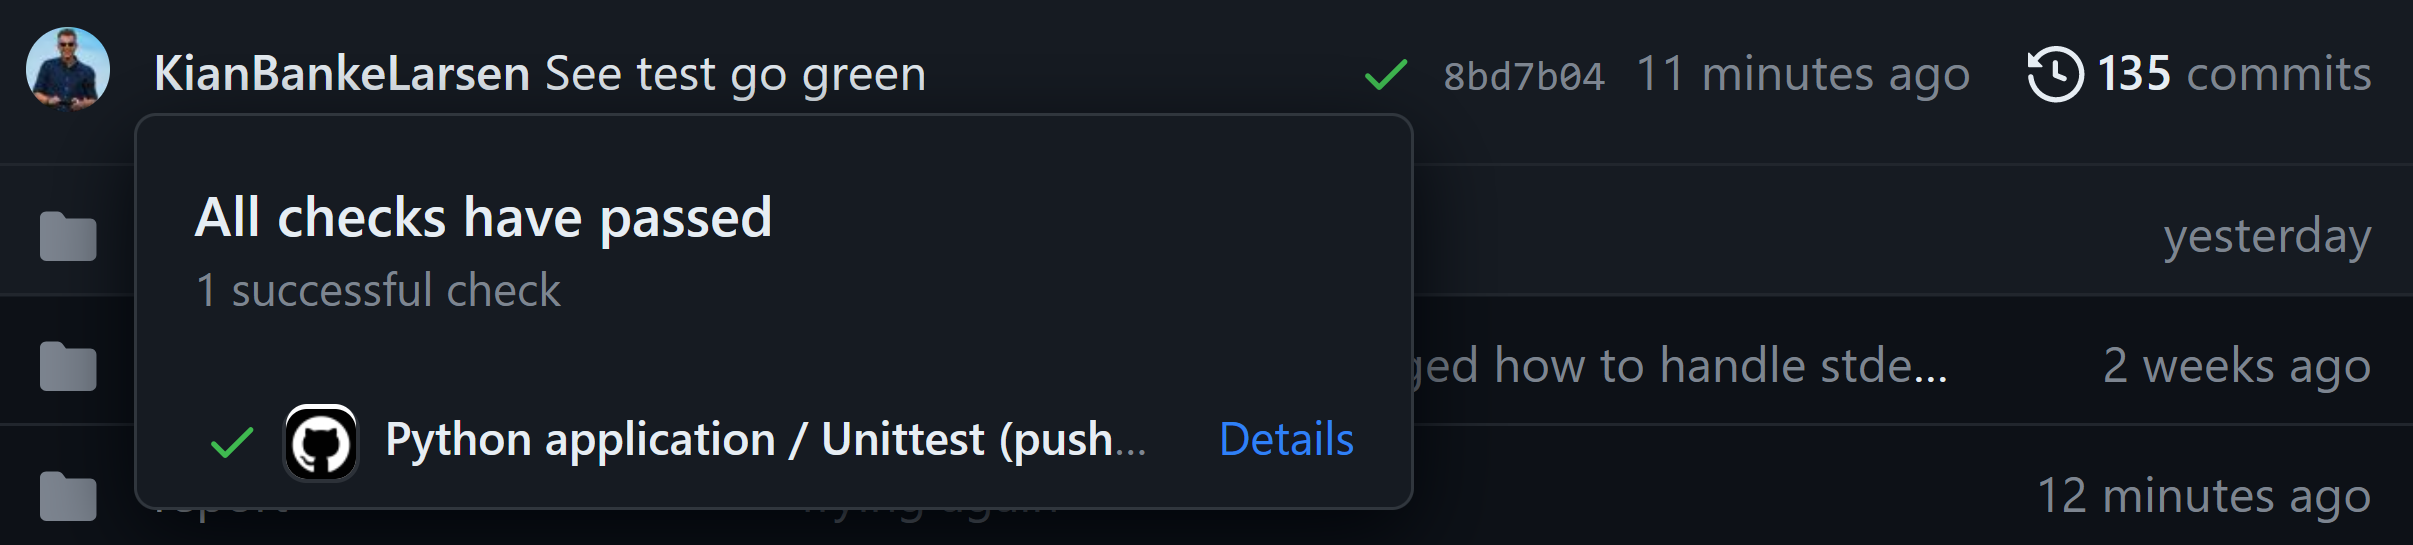
\includegraphics[width=1\textwidth]{misc/images/GitHub_Actions.png}
    \caption{GitHub Actions for system testing.}
\end{figure}

That way, one knows exactly which push or pull request caused the test to fail, and associated code is directly available from the workflow via commit ID. History for workflow is available too.

\begin{figure}[H]
    \centering
    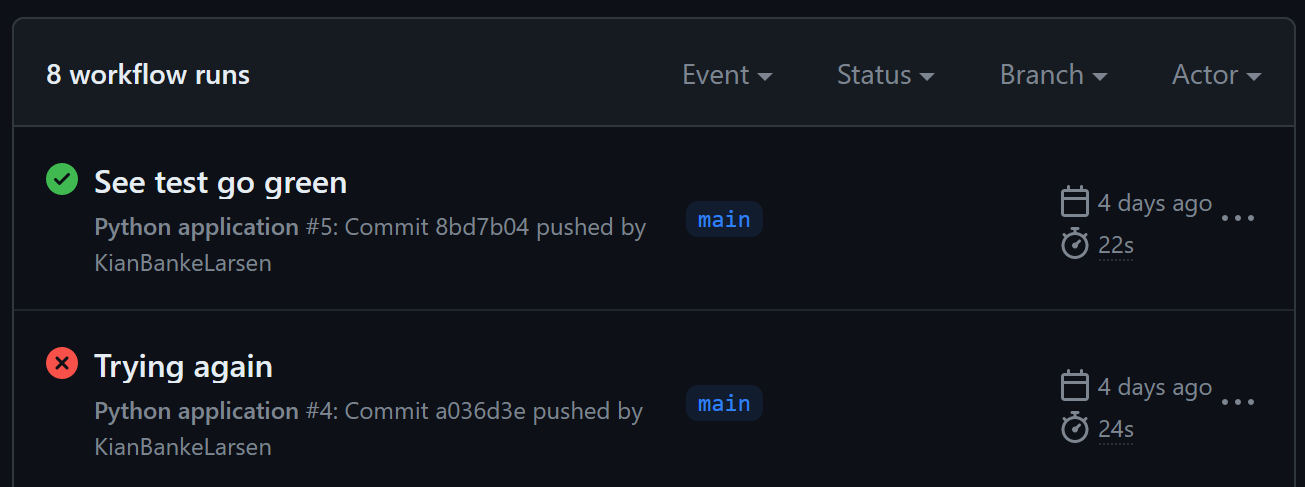
\includegraphics[width=1\textwidth]{misc/images/Workflow.png}
    \caption{Workflow history.}
\end{figure}

A workflow build consists of the stages stated in Figure \ref{fig:workflow_run}.  Note that, in this example, the stack machine test passed, but the register version did not. Upon build failure, an email is sent to whom introduced the issue (me).

\begin{figure}[H]
    \centering
    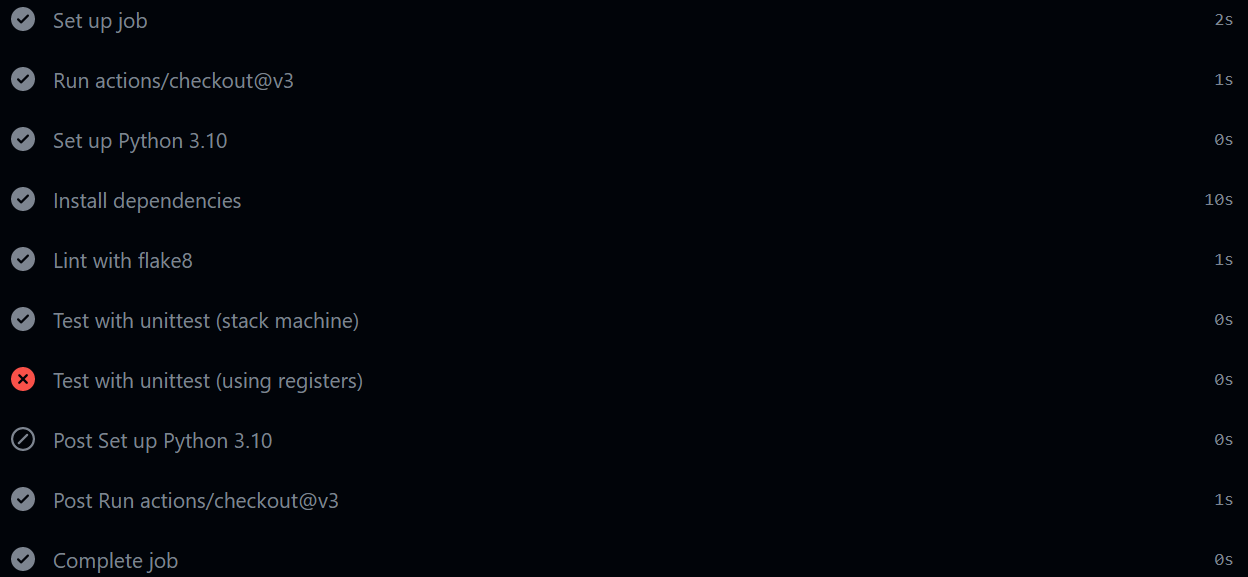
\includegraphics[width=1\textwidth]{misc/images/workflow_run.png}
    \caption{Workflow run. Red indicates failure.}
    \label{fig:workflow_run}
\end{figure}

The list of tests is too long to mention each one, instead three tests that caused particularly many problems have been chosen. The tests are representative because they have a relatively high complexity, as the input programs utilize recursion, loops and nested scopes. For this to work properly, it requires that the constructs and static link pointer works correctly. In addition, it must be possible to tear down several stack frames at once, since every scope introduces a new stack frame. Failing to remove a stack frame properly causes problems in the \texttt{postreturn} and \texttt{epilog} phase, and in worst-case segmentation fault. 

The test below is borrowed from SCIL. The test is named \texttt{summers.panda}.

\begin{minted}{c}
int sum_recurse(int n) {
    if(n == 1) {return 1;} else {
        return n + sum_recurse(n - 1);
    }
}
int sum_loop(int n) {
    int sum, i;
    i = 1; sum = 0;
    while(i <= n) {
        sum = sum + i;
        i = i + 1;
    }
    return sum;
}

print(sum_recurse(9)); print(sum_loop(9));
print(sum_recurse(42)); print(sum_loop(42));
\end{minted}

The test below does not calculate anything meaningful or difficult, but it checks that the functionality implemented in Figure \ref{fig:remove_stack_frames} works as expected.

\begin{minted}{c}
int i = 5;
int main(){
    if(1){
        if(1){
            if(1){
                i = i + 1;
                return i;
            }
        }
    }
}
print(main());
\end{minted}

The goal has been to test all legal semantics thoroughly. This includes assignment to variables declared outside the current scope. Assignment to formal parameters, recursion, return from static nested scopes, comments, sugared declaration with assignment, binary operations (comparisons and arithmetic) and constructs like \texttt{while}, \texttt{for}, \texttt{if} and \texttt{print}.

A test that is particularly critical for the register machine is right-unbalanced trees,\footnote{This is tested with the test cases \texttt{/testing/test-cases/unbalanced\_right\_addition.panda} and \texttt{/testing/test-cases/unbalanced\_right\_subtraction.panda}.} or complete trees, because these cause a greater register need. An example of such tree can be found in Figure \ref{fig:unbalanced_tree}. The figure is part of the syntax tree for the input program given below:

\begin{minted}{c}
print(1+(1+(1+(1+(1+(1+(1+(1+(1+(1+(1+(1+(1+(1))))))))))))));
\end{minted}

The reason is, in this case, that the left child is always visited first, after which the expression in the right child must be evaluated. This is clear in Figure \ref{fig:binop}. It is therefore necessary to preserve all left children until there are no more right children. This is not a concern applicable to the stack machine, as the stack just grows as expected. With register allocation, attention is required, because there must be a place to store values, since these must be in a register, regardless of whether this register is spilled onto the stack, it is still a ``register".

\begin{figure}[H]
    \centering
    \digraph[scale=0.5]{rightTree}{
	3 [label=1]
	4 [label=1]
	5 [label=1]
	6 [label=1]
	7 [label="..."]
	8 [label="+"]
	8 -> 6
	8 -> 7
	9 [label="+"]
	9 -> 5
	9 -> 8
	10 [label="+"]
	10 -> 4
	10 -> 9
	11 [label="+"]
	11 -> 3
	11 -> 10
	12 [label=print]
	12 -> 11
}

    \caption{Unbalanced expression.} 
    \label{fig:unbalanced_tree}
\end{figure}

To be precise, the input program uses 27 temporary registers as a consequence of the code generation, which after preparation of the interference graph and coloring can be stored in 14 physical registers. The Emit phase only provides 9 registers for storage, meaning that 5 registers are located on the stack.


\section{Coverage}
Coverage cannot and should not be a measure of test quality, because the order in which functions and flow are executed has a great influence on the result. However, code coverage gives a direct warning if subsets of the code have not been tested at all. Thus, it is clear that more tests need to be written.

The code coverage measuring tool \texttt{coverage.py} is used to perform code coverage statistics on this project. Code coverage is performed in the following way:

\begin{minted}{text}
Compiler$ python3.10 -m coverage erase
    && python3.10 -m coverage run -a main.py -td
    && python3.10 -m coverage run -a main.py -tsd 
    && python3.10 -m coverage report 

Name                                     Stmts   Miss  Cover
------------------------------------------------------------
main.py                                     24      2    92%
src/compiler.py                             70      3    96%
src/dataclass/AST.py                       125      0   100%
src/dataclass/iloc.py                       22      0   100%
src/dataclass/symbol.py                     36      2    94%
src/enums/code_generation_enum.py           38      0   100%
src/enums/symbols_enum.py                    5      0   100%
src/phase/allocator.py                     213      5    98%
src/phase/code_generation_base.py           58      3    95%
src/phase/code_generation_register.py      262      9    97%
src/phase/code_generation_stack.py         199      5    97%
src/phase/emit.py                          205     20    90%
src/phase/lexer.py                          44      8    82%
src/phase/parser.py                        101      2    98%
src/phase/parsetab.py                       18      0   100%
src/phase/symbol_collection.py             117      2    98%
src/phase/syntactic_desugaring.py           65      0   100%
src/printer/ast_printer.py                 141      3    98%
src/printer/generic_printer.py              17      0   100%
src/printer/symbol_printer.py               40      0   100%
src/utils/error.py                           5      0   100%
src/utils/interfacing_parser.py              1      0   100%
src/utils/label_generator.py                 7      0   100%
src/utils/x86_instruction_enum_dict.py       2      0   100%
testing/test.py                             75      0   100%
------------------------------------------------------------
TOTAL                                     1890     64    97%
Wrote HTML report to htmlcov/index.html
\end{minted}

Based on this output, it can be assessed that the prepared tests in the \texttt{test-cases} folder cover the code well. Note that code coverage is run with the debug flag, \texttt{-d}. This is because code in the printer files are only executed when debug is desired.

It is possible to convert the coverage data to an HTML report with the command \texttt{python3.10 -m coverage html}. The advantage of having the data in report form is that it is possible to see which lines have been executed and which are missing, as shown in the figure below: 

\begin{figure}[H]
    \centering
    \begin{subfigure}{1\textwidth}
        \centering
        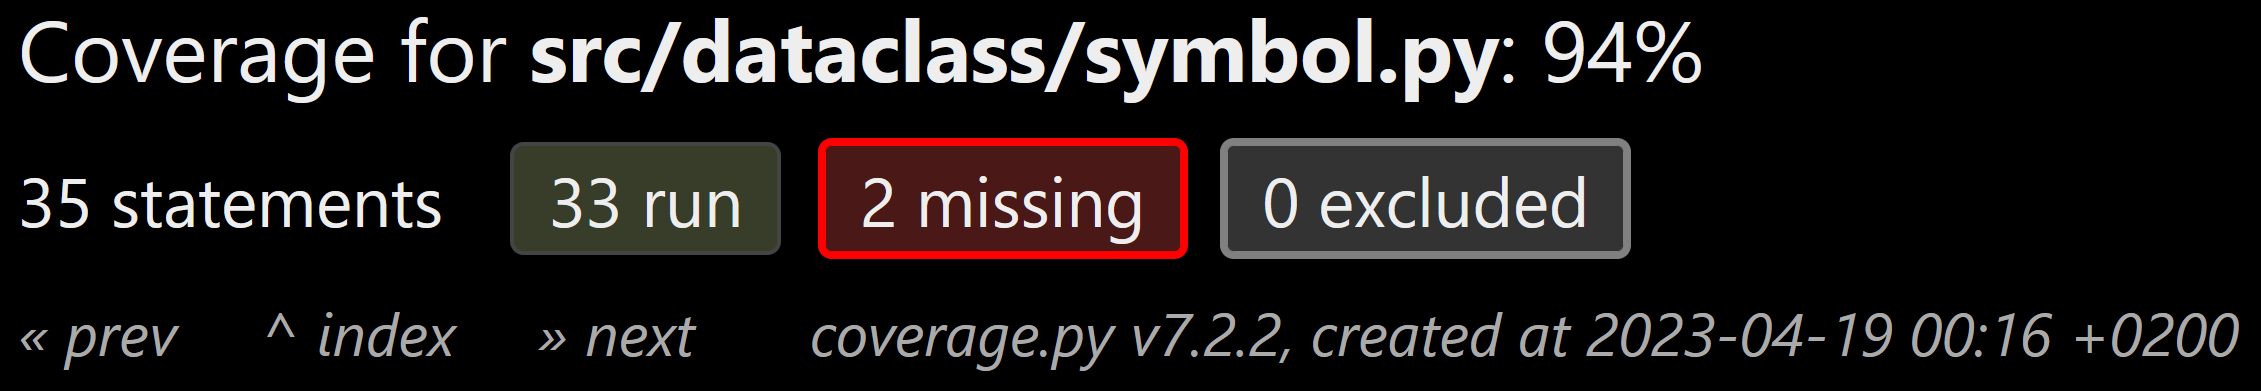
\includegraphics[width=1\textwidth]{misc/images/Coverage_Panel.png}
        \end{subfigure}\\
        \begin{subfigure}{1\textwidth}
        \centering
        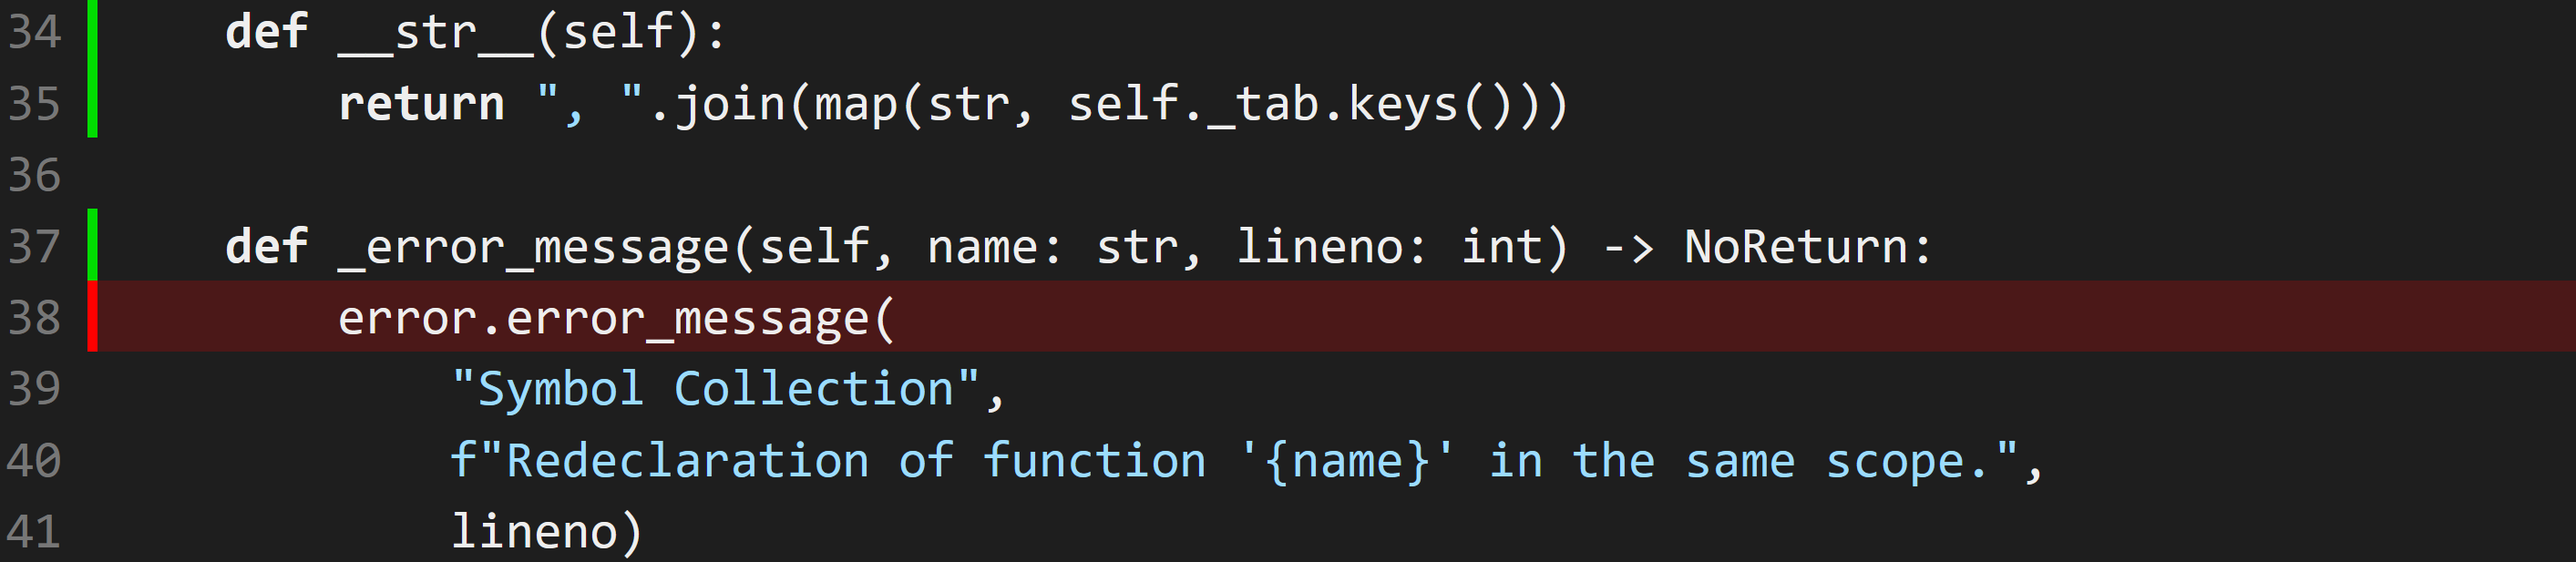
\includegraphics[width=1\textwidth]{misc/images/Coverage_Info.png}
        \end{subfigure}
    \caption{Coverage HTML report.}
\end{figure}

The HTML report also makes it possible to carry out filtering etc. in the file overview table, and thus get a nicer and more user-friendly interface, Figure \ref{fig:cov_report}.

\begin{figure}[H]
    \centering
    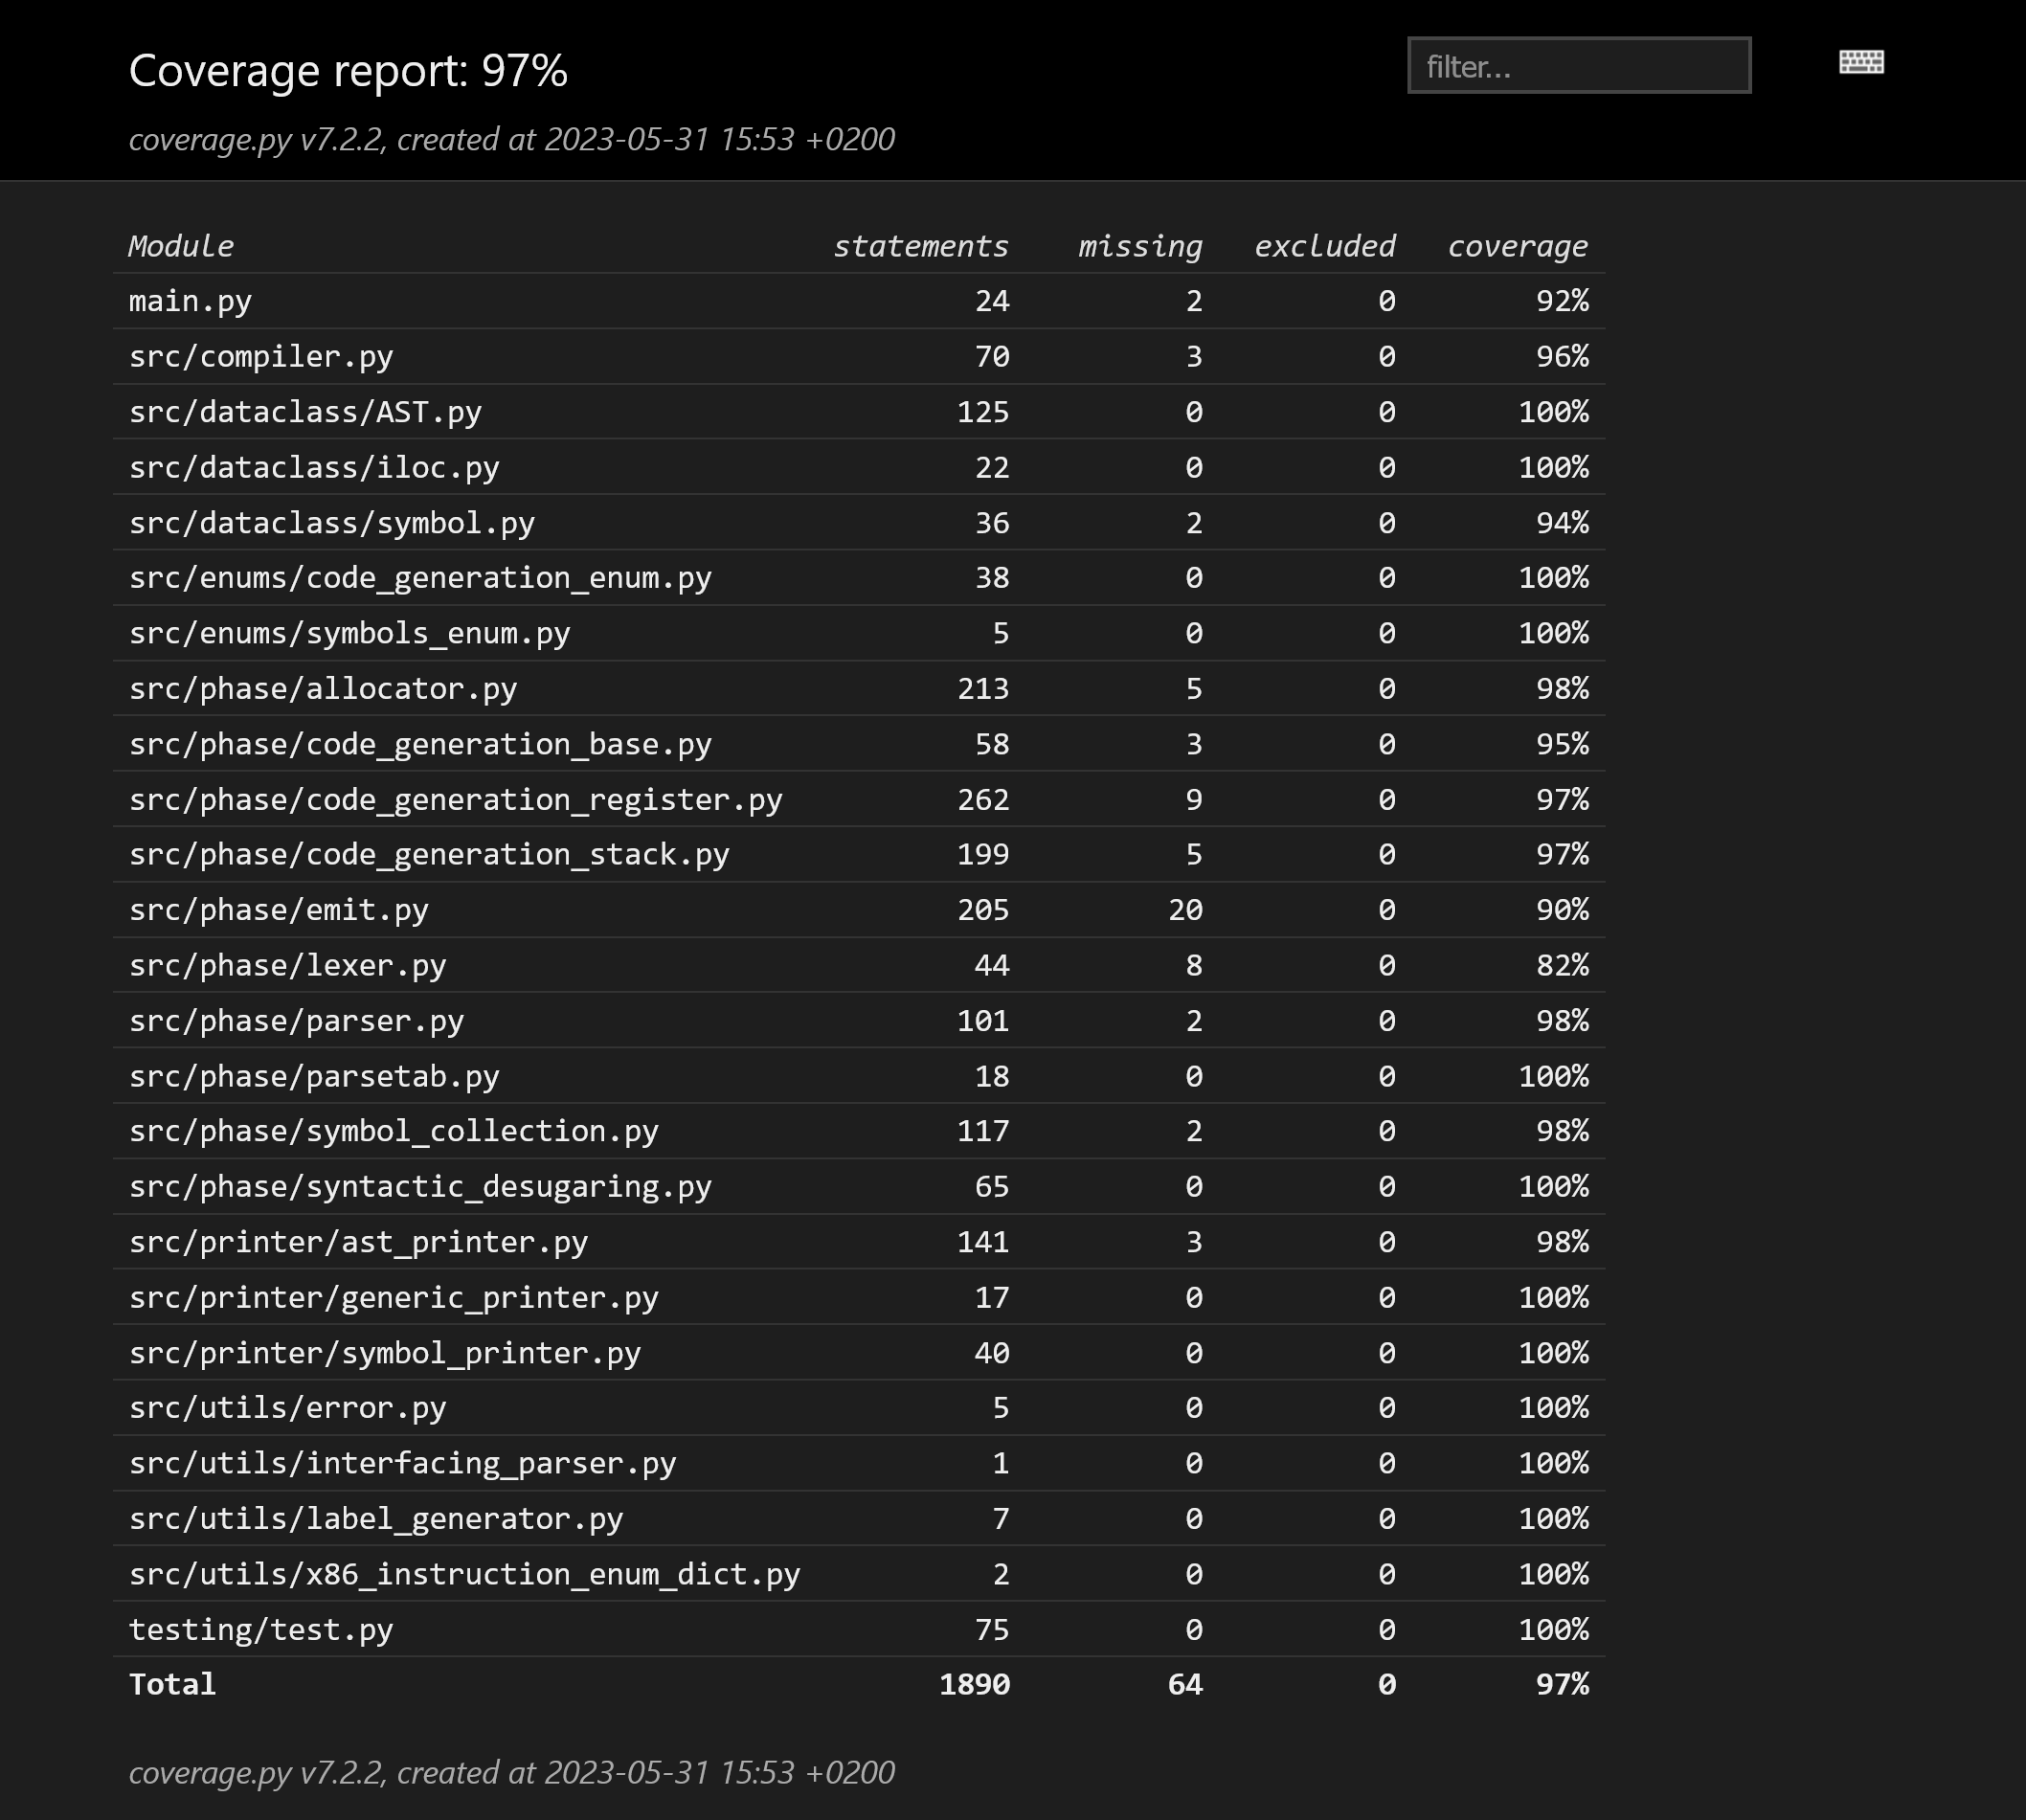
\includegraphics[width=1\textwidth]{misc/images/Coverage_report.png}
    \caption{Coverage report.}
    \label{fig:cov_report}
\end{figure}

\chapter{Performance Comparison}
It is time to compare the performance of the stack machine and the register machine. Only the three tests indicated in Figure \ref{fig:performance_comparison} have been made, as it is limited how many tests can be made without composite types. The tests are:

\begin{itemize}
    \item \texttt{sum\_loop} from \texttt{test-cases/summers.panda} called with actual parameter $300000000$.
    \item \texttt{fib} from \texttt{test-cases/fibonacci\_classic.panda} called with actual parameter $39$.
    \item \texttt{for}-loop performing $500000000$ iterations of adding two numbers.
\end{itemize}

All test results are calculated as an average of 10 measurements. The tests have been performed on an Intel x86 Core i9-8950HK Coffee Lake Processor, and timed using the native tool \texttt{time} in Ubuntu (based on \texttt{real} time).

Not much performance gain was expected by using the register machine versus the stack machine, since the register allocation is rather limited. One might even have expected slower executions because values move between more physical registers than necessary (peep-hole optimization required). A remarkable performance gain is observed for all tests when using the register machine.

The reason for the increased performance of the register machine is, by hypothesis, due to the use of move instructions despite push and pop instructions. Based on a scientific paper written by Agner Fog from DTU, \cite[314-315]{instruction}, the hypothesis is not without authority. Figure \ref{tab:instruction_table} presents a table comparing reciprocal throughput. Without getting too technical and analytical about the compiled programs, we achieve approximately 50\% better performance by replacing push and pop instructions with move instructions. It agrees very well with the performance gain we see in \texttt{sum\_loop}. It is expected that Fibonacci is dominated by the complexity associated with handling stack frames, and therefore we do not achieve the same performance gain. The result in the \texttt{for}-loop test is remarkable, but the primary work is also optimized from a reciprocal throughput of almost $1$ to around $0.25$. The tests are satisfactory, and we conclude that the hypothesis holds.

% python3.10 main.py -f ../performance/for-loop.panda -cs
% time ./src/output/a.out

\begin{figure}[h]
    \centering
    \pgfplotstableread[row sep=\\,col sep=&]{
test & stack & register \\                                         
%sum\_recurse(30000) & 21 & 21 \\                                          
sum\_loop(300000000) & 1461 & 858 \\                                         
fibonacci(39) & 2159 & 1648 \\                                                                              
for-loop & 2361 & 852 \\                     
}\mybardata
\begin{tikzpicture}
    \begin{axis}[
        ybar,
        ylabel=Milliseconds,
        ymajorgrids=true,
        xtick pos=lower,
        %xticklabel style={rotate=90},
        %ytick pos=left,
        grid style=dashed,
        width=1\linewidth,
        xlabel=Test,
        title = Milliseconds vs Test,
        bar width=.6cm,
        legend style={at={(0.05,.95)},anchor=north west},
        symbolic x coords={sum\_loop(300000000),fibonacci(39), for-loop},
        xtick=data,
    ]
    \addplot+[color=blueplot] table[x=test,y=register]{\mybardata};
    \addplot+[color=redplot] table[x=test,y=stack]{\mybardata};
    \legend{Register, Stack}
    \end{axis}
\end{tikzpicture}
    \caption{Stack Machine vs Register Machine.}
    \label{fig:performance_comparison}
\end{figure}

\begin{table}[h]
    \centering
    \begin{tabular}{l|c|c}
        Instruction  & Operands &  Reciprocal throughput \\ \hline
        MOV & r,i & 0.25 \\\hline
        MOV & r32/64,r32/64 & 0.25\\ \hline
        MOV & r32/64, m & 0.5 \\\hline
        PUSH & r & 1 \\\hline
        PUSH & i & 1 \\\hline
        PUSH & m & 1 \\\hline
        PUSH & stack pointer & 1 \\\hline
        POP & r & 0.5 \\\hline
        POP & stack pointer & 3 \\\hline
        POP & m & 1
    \end{tabular}
    \caption{Coffee Lake integer instructions.}
    \label{tab:instruction_table}
\end{table}

\chapter{Evaluation}
This chapter is devoted to reflecting on the learning through the project, as well as describing some issues that could be interesting to work on if the project had had a longer duration.

\section{Retrospect}
There are two fundamental principles that must be observed when building a compiler. The first principle is inviolable:

\begin{displayquote}
    \textit{``The compiler must preserve the meaning of the input program.''}
\end{displayquote}
\hspace*\fill{\small--- \cite[6]{EnginneringACompiler}}

The second principle has a more practical aspect:

\begin{displayquote}
    \textit{``The compiler must discernibly improve the input program.''}
\end{displayquote}
\hspace*\fill{\small--- \cite[7]{EnginneringACompiler}}

It has been a core value throughout the project to make a well-defined compiler implementation that does not do anything inappropriate. Furthermore, the goal has been to create a clear, consistent, easily understandable grammar that a user would be able to pick up with ease. It is assessed that the first principle has been complied with. In this project, no special effort has been made in optimization apart from the preparation of an implementation that uses registers, which is why the second principle must be trivially respected. An example of an optimization that could challenge this would be instruction scheduling, since instructions are literally rescheduled after the invariant based linear IR has been generated.

The approach to the project has been academically based on literature, in order to gain an overview of new as well as old knowledge. Although this has given a confident approach to the project, it must be recognized that it has dulled the process unnecessarily. When coding a project such as a compiler that consists of relatively many lines of code, and many hours of debugging, it is necessary to purposefully choose a theme and then learn as needed, otherwise many hours are lost on something that is not directly applicable. The hours are of course not wasted, but not beneficial for the project either.

It has always been desired that it should be possible to declare new variables in any scope, which is why it was decided to let \texttt{body} (syntactic category from parsing) be what constituted a scope. The choice later made it clear, during Code Generation phase, that this imposed too many constraints on how the stack should be set up, since a simple generalized procedure linkage was wanted. This resulted in suddenly having to handle all scopes as procedure calls, though it had nothing to with a procedure call. One also encounters problems when doing local register allocation, because flow is only considered locally for a scope (normally local to functions). This consequence limits the analysis to the individual scope, making the content of a \texttt{then} block, of an \texttt{if} statement, a black box for the surrounding scope. Thus, the analysis of control flow becomes less effective, which contributes to overall poorer performance of the register machine. The easiest solution, and most likely most effective, would be to redo the scope implementation. Global register allocation would be the hard option, though it would not solve the underlying problem besides patching it.

\section{Further Development}
The first thing to solve is the scope implementation. This is possibly where the greatest performance is to be gained, based on the compiler's current functionality. Being able to analyze flow for entire functions will make it easier to optimize the use of registers. Especially in the case of using variables outside the current scope, the variables will then be marked as \texttt{escaping}, which causes them to live on the stack, which is suboptimal when wanting to use registers. At present, loops cannot really benefit from registers, since we are unable to effectively reference variables located in external scopes.

Another challenge is that there is no \texttt{push imm64} instruction, which can cause the error: ``\texttt{Error: operand type mismatch for `push'}". The error occurs, for example, when a number greater than \SI{32}{bit} two's complement is printed, as the number to be printed will be pushed directly to the stack. This is suboptimal because the registers and the reserved stack space is \SI{64}{bit}, but we can efficiently only use \SI{32}{bit} at worst. A similar error apply to the register machine, as \texttt{movq} cannot handle immediate source operands larger than \SI{32}{bit} two's complement. Workarounds are available, but they enforce a more advanced implementation than prepared in this project. 

At present, all spilled registers are stored as temporary saves on the stack, but it might be desirable to move some spilled registers to the local data area and parameter area, so that the space already allocated on the stack is used efficiently.

Finally, it could be advantageous with composite data types like arrays to make the language Turing Complete -- it is not possible to calculate anything significant, as one can only work with integers and Boolean values ($0$ or $1$ integer). Composite data types will only further the potential of the already implemented programming constructs. Besides adding more types, it would be nice with a type-checking phase in the front end too.


\section{Single Point of Contact}
As a final rounding and summary of the project, GitHub Pages has been used as an addendum to the report, hoping to provide a brief user-friendly introduction to the code and the report. A screenshot of the website can be found in Figure \ref{fig:GitHub_Pages}.

The website has been created with Jekyll, which is a tool that can automatically transform plain text into a static website. The tool only requires a small YAML file (\texttt{/\_config.yml}), listed below, and a markdown file for the page's content.

\begin{minted}{yaml}
theme: jekyll-theme-slate
title: Panda Compiler
description: This is a bachelor project, Southern University of Denmark
show_downloads: true
\end{minted}

The website is simply a nice presentation of the \texttt{README.md} file. In addition, it is possible to download the project directly here, or follow the link to GitHub.

\begin{figure}[H]
    \centering
    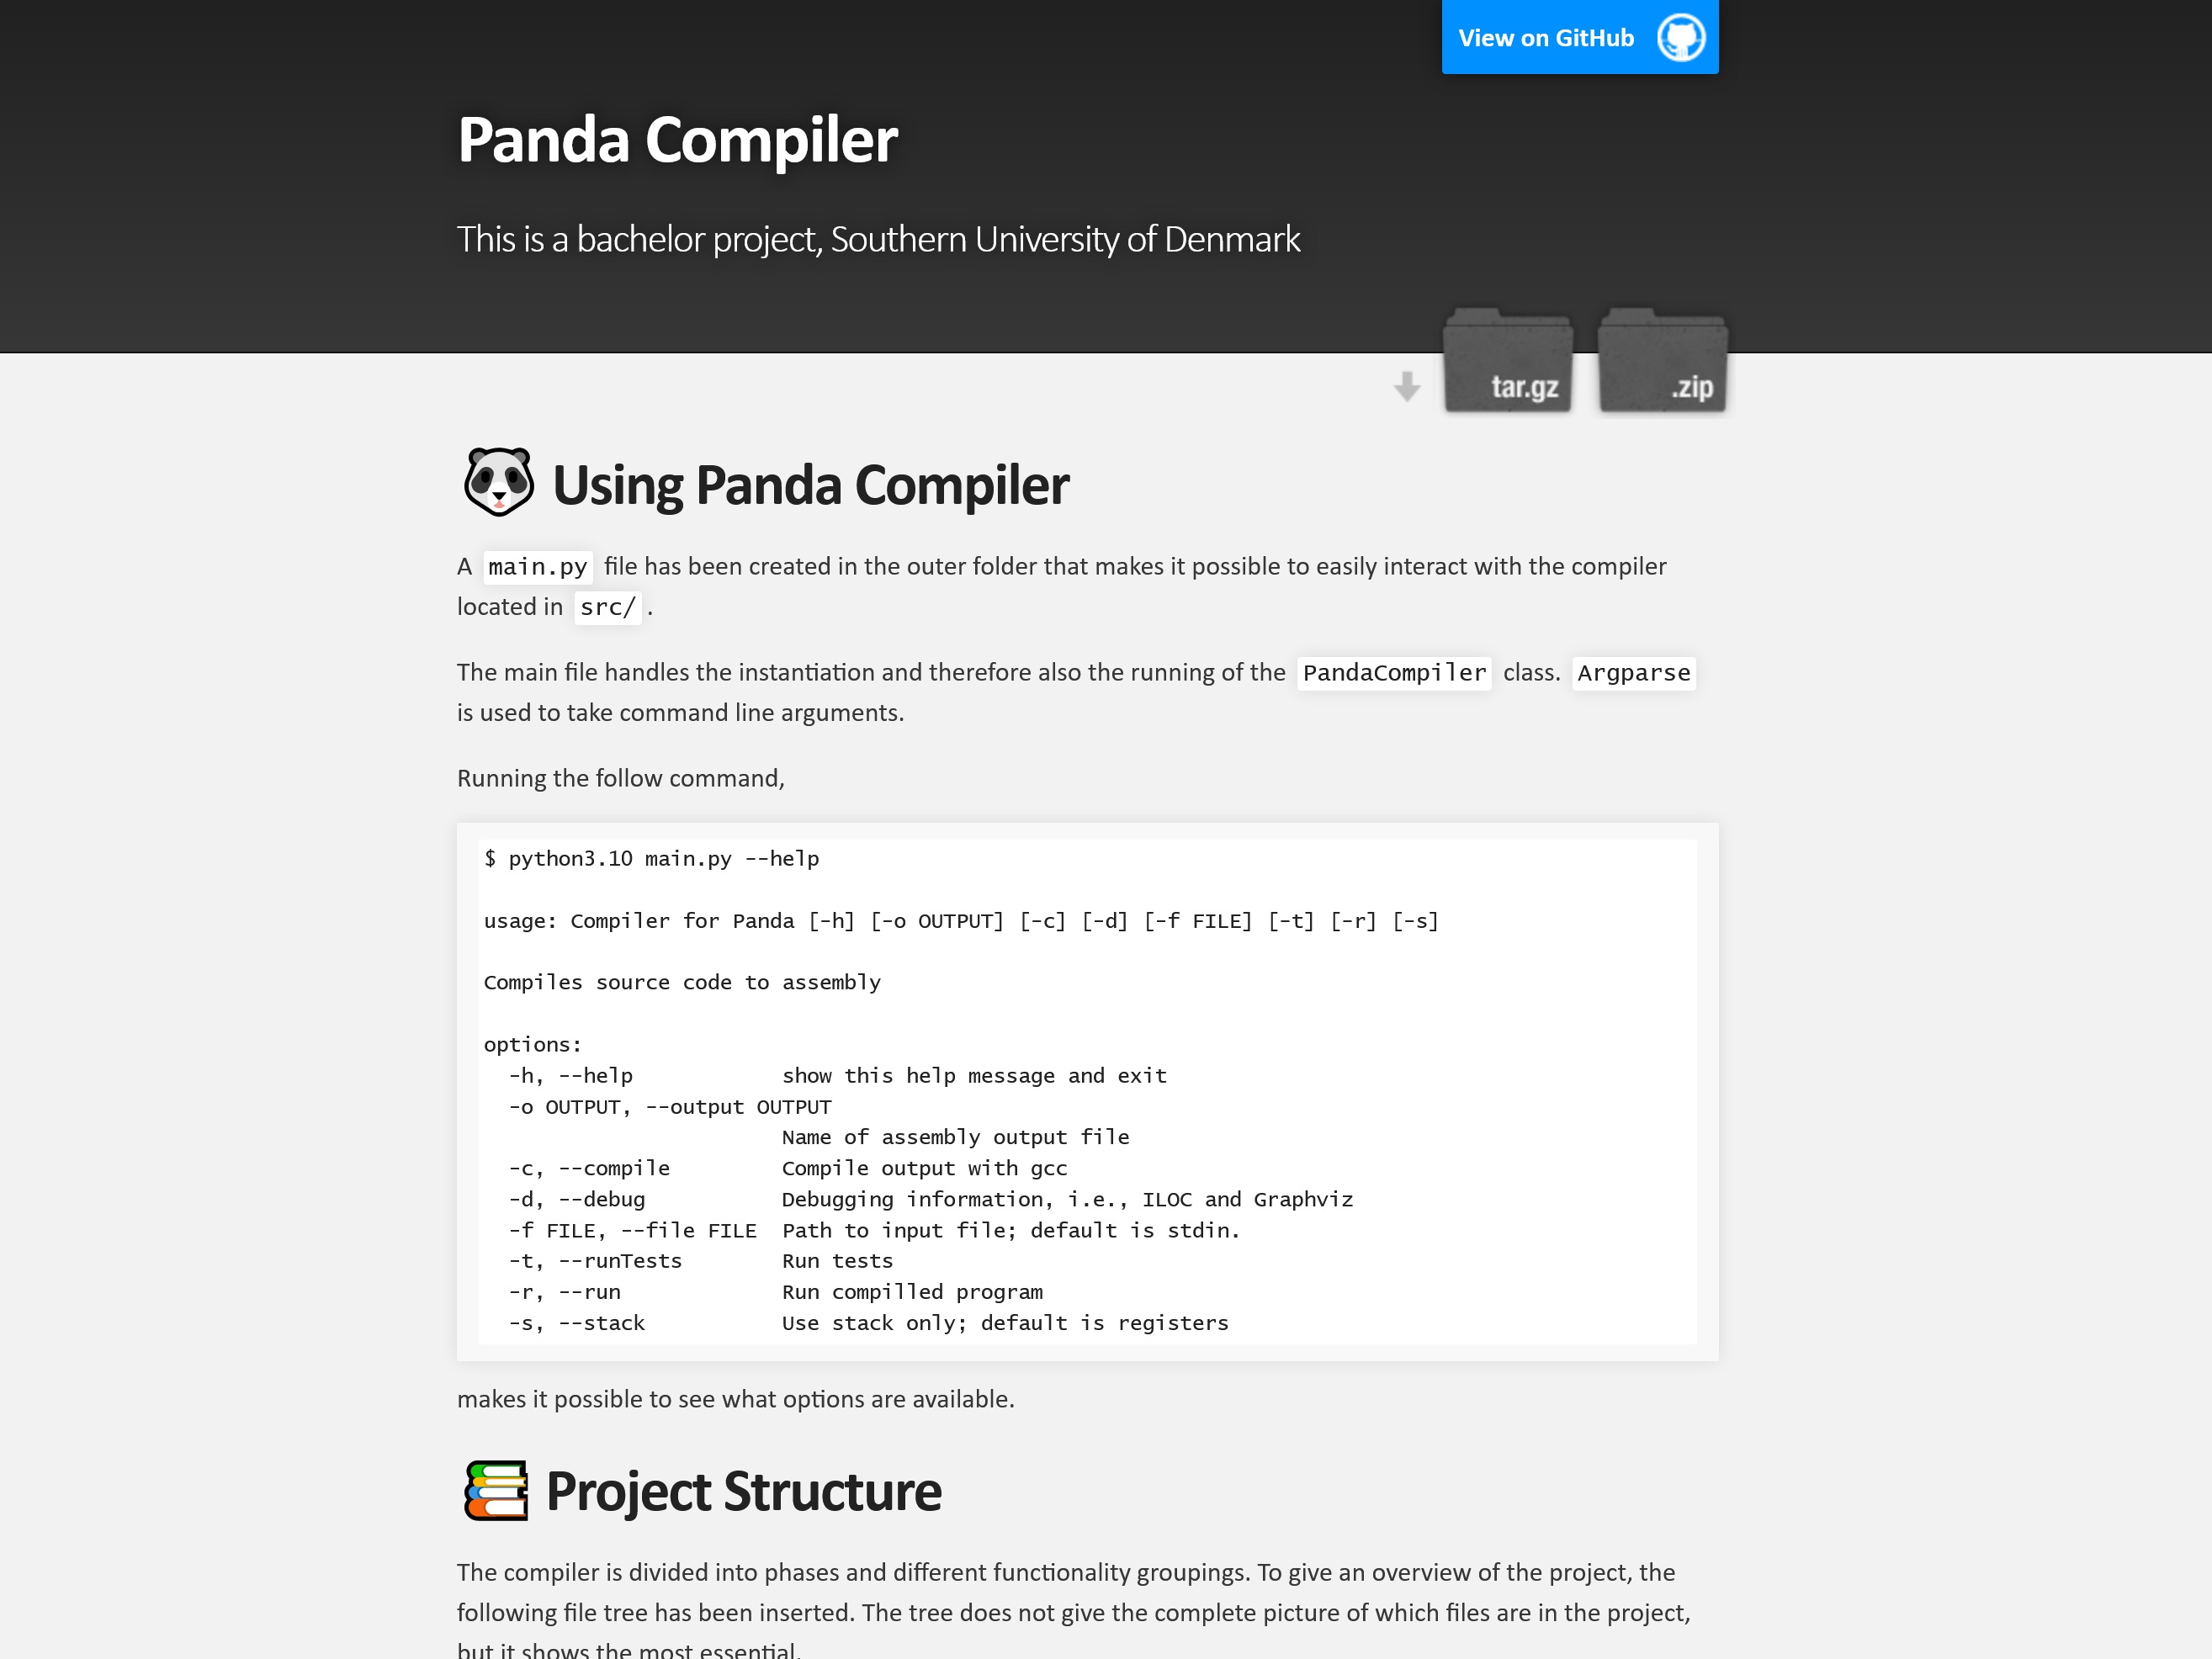
\includegraphics[width=1\textwidth]{misc/images/GitHub_Pages.png}
    \caption{Automatically generated Jekyll Slate website hosted on GitHub Pages: \url{https://kianbankelarsen.github.io/Compiler/}.}
    \label{fig:GitHub_Pages}
\end{figure}

GitHub Pages takes care of deployment when a YAML is specified. Subsequently, the website will be automatically deployed on any push to GitHub -- at the same time as the workflow for testing runs.

\chapter{Conclusion}
In this bachelor project, a compiler has been successfully implemented, which can be used both as a stack machine and as a register machine. The compiler consists of a scanner, parser, symbol collector, desugar-class, code generator, allocator and a code emitter. The compiler consists of approximately 3500 lines of Python code.

The implemented language is named Panda, and resembles a subset of C. The implemented types are Boolean and integer (actually both are integers). Constructions such as \texttt{if}-\texttt{else} statements, \texttt{while}-loops and \texttt{for}-loops have also been implemented. \SI{64}{bit} are used for all types of values. It had been well regarded with composite types, such as arrays, but unfortunately, it was not achieved in the time frame.

The performance of the stack machine and the register machine have been compared, and it turns out that the register machine runs remarkably faster, which is a very satisfactory result. Depending on the given test, a performance gain of up to a factor of three is observed.

Correctness of the compiler has been tested using 25 test cases and all tests run successfully. Furthermore, a workflow has been set up to carry out these tests via GitHub Actions, which ensures that all code pushed to production is tested. In the event of an error, the person responsible will receive a notification accordingly. Although the 25 tests do not provoke an error, this does not mean that the compiler does not contain any errors, just that they have not been discovered yet. The 25 tests achieve a code coverage of 97\%, which is sufficient.

Every project has a README. In addition to introducing the project, a static website has been generated on the file, from which the code is publicly available: \url{https://kianbankelarsen.github.io/Compiler/}

The implementation of scopes is not optimal, which is why it could be interesting to refactor, given that there was more time to work on the project. Only when this is done will it be possible to fully utilize the register allocation, and in that way, achieve an even greater performance gain.

\cleardoublepage
\phantomsection
\addcontentsline{toc}{chapter}{References}
\printbibliography
\end{document}